\documentclass[12pt]{article}
\usepackage{fontspec}
\setmainfont{Times New Roman}
\usepackage[legalpaper,margin=0.8in]{geometry}
\usepackage{xcolor}
\usepackage{amsmath}
\usepackage{graphicx}
\usepackage{caption}
\usepackage{longtable} % For long tables spanning multiple pages
\usepackage{array}
\usepackage{makecell}
\usepackage{setspace}
\onehalfspacing % Για απόσταση $1.5$ γραμμών
\usepackage{pgfplots}
\pgfplotsset{compat=1.17}
\usepackage{pgfplotstable} 
\usepackage{booktabs}
\usepackage{caption}
\usepackage{hyperref} % For hyperlinks
% \usepackage[utf8]{inputenc} % removed for XeLaTeX compatibility % Encoding
\usepackage[ruled,vlined]{algorithm2e}
\usepackage{babel}
\usepackage{amsfonts} % Provides \mathbb{} for number sets
\usepackage{bm}       % Proper bold math symbols with \bm{}

\title{Η απόδοση των μαθητών λαμβάνοντας υπόψη παράγοντες της καθημερινότητας τους}




\author{Ιωάννου Νικόλας - ge20718 
\\ Μπέκος Θοδωρής - ge20034}
\date{Δεκέμβριος 2024}


\begin{document}
\sloppy
\maketitle

\vspace{0.7cm}
\begin{center}
    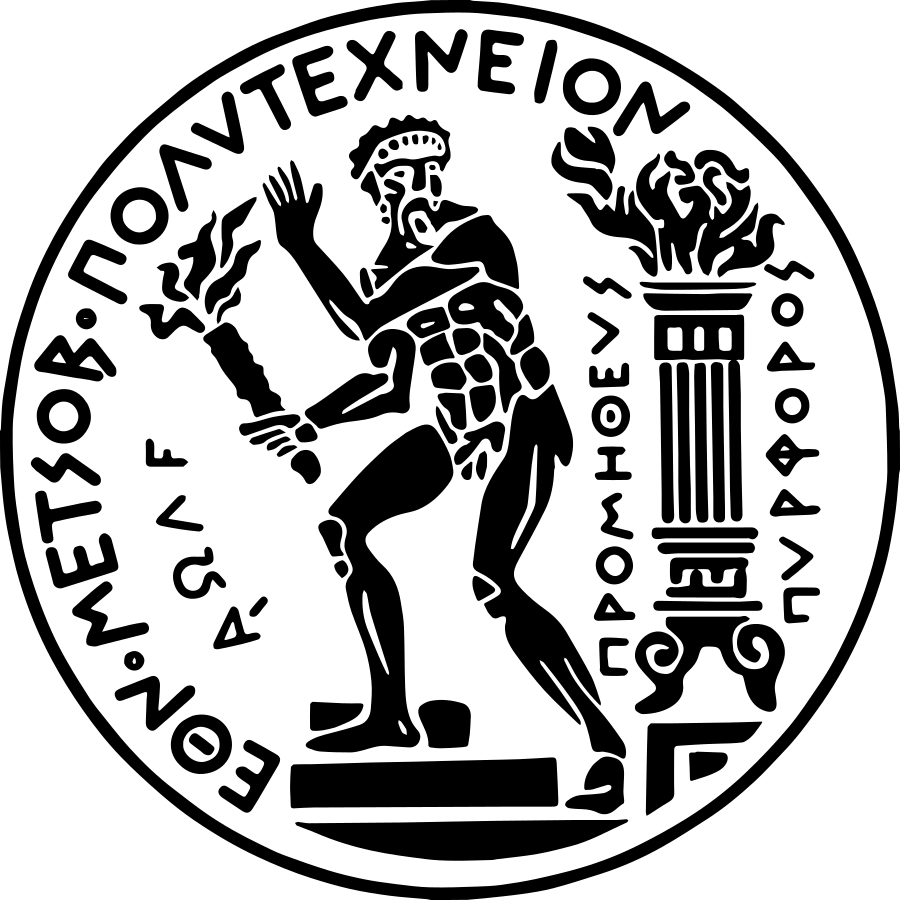
\includegraphics[width=0.7\textwidth]{./images/Εθνικό_Μετσόβειο_Πολυτεχνείο.svg}
    
    \Large Σχολή εφαρμοσμένων μαθηματικών και φυσικών επιστημών \\[1.5cm]
\end{center}



        
\vfill


        \noindent Μάθημα: ΘΕΜΑ \\[0.5cm]


        \noindent\textbf{Υπέυθυνος καθηγητής:} 
        Δρ. Στεφανέας Πέτρος \\[1cm]

\newpage
\noindent\textbf{Ευχαριστίες:} \\

\noindent Θα θέλαμε να ευχαριστήσουμε τον κύριο Πέτρο Στεφανέα για το ενδιαφέρον και
την εμπιστοσύνη που μας έδειξε κατά τη διάρκεια πραγματοποίησης της εν λόγω εργασίας. Επίσης, θα θέλαμε να ευχαριστήσουμε τις οικογένειες μας γιατί χωρίς αυτές δεν θα μπορούσαμε να βρισκόμασταν στη θέση που βρισκόμαστε τώρα.

\newpage
\renewcommand{\contentsname}{\Huge \textbf{Περιεχόμενα}}

% Πίνακας περιεχομένων
\tableofcontents
\newpage

\section{Εισαγωγή}
km \\
\newpage

\section*{Introduction}
gt \\
\newpage
\section{Ανάλυση της διαδικασίας επιλογής μοντέλου}
\subsection{Ανάλυση του προβλήματος}

\noindent Το πρόβλημα το οποίο αντιμετωπίσαμε είχει να κάνει με την δημιουργία ενός μοντέλου μηχανικής μάθησης για την εκτίμηση των βαθμών που θα επιτύχουν οι μαθητές στην εξέταση ενός μαθήματος , μέσω διαφόρων παραγόντων που θα αναλύσουμε παρακάτω. Το πρόβλημα αυτό αποτελεί πρόβλημα παλινδρόμισης αφού ο τελικός βαθμός δεν αποτελεί κατηγορική αλλά ποσοτική μεταβλητή και παίρνει συνεχείς τιμές. Χρησιμοποιήσαμε το σύνολο δεδομένων  Student Performance Factors που βρήκαμε στο Kaggle, όπου τα χαρακτηριστικά τα οποία το αποτελούν φαίνονται στον πίνακα παρακάτω:\\

\begin{center}
\begin{longtable}{|p{5cm}|p{7.1cm}|p{4cm}|} % Creates a table with 3 columns, all centered, with borders
\hline
Χαρακτηριστικά & Περιγραφή & Εύρος τιμών \\ % Header row
\hline
Attendance & \makecell[l]{Ποσοστό μαθημάτων που\\ παρευρέθηκε ο μαθητής} & 0-100 \\ % Row 1
\hline
Previous Scores & \makecell[l]{Μέσος όρος βαθμών απο\\ προηγούμενες εξετάσεις} & 0-100 \\ % Row 7
\hline
Sleep Hours & \makecell[l]{Ώρες ύπνου ανά μέσο όρο\\ κάθε βράδυ} & 4-10 \\ % Row 6
\hline
Hours Studied & Αριθμός ωρών που δίαβασε ο μαθητής μέσα στην βδομάδα & 0-50 \\ % Row 2
\hline
Tutoring Sessions &\makecell[l]{Αριθμός φροντιστηριακών\\ μαθημάτων ανά μήνα} & 0-10 \\ % Row 10
\hline
Family income & Οικογενειακό εισόδημα & Low/Medium/ High \\ % Row 11
\hline
Teacher quality & \makecell[l]{Εκπαιδευτική ικανότητα\\ καθηγητή} & Low/Medium/ High \\ % Row 12
\hline
\makecell[l]{Parental\\ Involvement} & \makecell[l]{Βαθμός εμπλοκής γονέων\\ στην εκπαίδευση του μαθητή} & Low/Medium/ High \\ % Row 3
\hline
Access to Resources & \makecell[l]{Πρόσβαση μαθητή σε\\ εκπαιδευτικό υλικό} & Low/Medium/ High \\ % Row 4
\hline
Motivation Level & Κίνητρο μαθητή & Low/Medium/ High \\ % Row 8
\hline
Peer Influence & \makecell[l]{Επιρροή που δέχεται ο\\ μαθητής απο ομήλικους του} & \makecell[l]{Negative/\\ Neutral/ \\Positive} \\ % Row 14
\hline
Distance from home & Απόσταση σχολείου απο το σπίτι & Near/Moderate/ Far \\ % Row 18
\hline
School type & Τύπος σχολείου & Private/Public \\ % Row 13
\hline

Physical activity & \makecell[l]{Επίπεδο φυσικής \\ δραστηριότητας μαθητή} & \makecell[l]{Sedentary/ \\ Light/Moderate/ \\ Active/ \\ Very Active/ \\ Highly Active/ \\ Athlete} \\ % Row 15
\hline

\makecell[l]{Parental education \\level} & Επίπεδο εκπαίδευσης γονέα & \makecell[l]{High School/ \\ College/ \\ Postgraduate} \\ % Row 17
\hline
Extracurricular activities & Εξωσχολικές δραστηριότητες & Yes/No \\ % Row 5
\hline
Learning disabilities & Μαθησιακές δυσκολίες & Yes/No \\ % Row 16
\hline

Internet Access & Πρόσβαση στο διαδίκτυο & Yes/No \\ % Row 9
\hline
Gender & Φύλο μαθητή & Male/Female \\ % Row 19
\hline

Exam Score & Βαθμός εξέτασης & 0-100 \\ % Row 20
\hline
\end{longtable}
\end{center}

Η μεταβλητή Exam Score αποτελεί την εξαρτημένη μεταβλητή(μεταβλητή στόχο) του μοντέλου ενώ οι υπόλοιπες μεταβλητές αποτελούν τις πιθανές ανεξάρτητες μεταβλητές. 


\subsection{Επεξεργασία των δεδομένων}
Ρίχνωντας μια ματιά στα δεδομένα παρατηρήσαμε πως υπάρχουν παρατηρήσεις με ελλειπείς τιμές. Στην συγκεκριμένη περίπτωση έχουμε 3 επιλογές. Η πρώτη επιλογή ήταν να διαγράψουμε τις παρατηρήσεις αυτές, η δεύτερη να προβλέψουμε τις τιμές των παρατηρήσεων με κάποια μέθοδο (Παλινδρόμιση για τις ποσοτικές και ομαδοποίηση για της κατηγορικές μεταβλητές) και η τρίτη να αντικαταστήσουμε τις ελλειπείς τιμές με κάποιο λογικό τρόπο(π.χ. εάν έχουμε ποσοτικές τιμές με την μέση τιμή του χαρακτηρηστικού ή εάν έχουμε κατηγορική με την τιμή, η οποία εμφανίζεται τις περισσότερες φορές). Επιλέξαμε να διαγράψουμε τις παρατηρήσεις οι οποίες έχουν ελλειπείς τιμές μιας και ο αριθμός των παρατηρήσεων είναι ικανοποιητικός και οι ελλειπεις τιμές αποτελούν ένα πολύ μικρό ποσοστό(<10\(\%\)) των συνολικών παρατηρήσεων και δεν θα επιρεάσουν το αποτέλεσμα. 

Η μεταβλητή Physical Activity εχει μια ιδιαιτερότητα. Παρόλο που περιλαμβάνει αριθμητικές τιμές(0-6), αυτές οι τιμές αποτελούν κατηγορίες. Για αυτό και εμείς αλλάξαμε τον τύπο της μεταβλητής σε αντικείμενο. Εύκολα μπορούμε να δούμε πως το dataset μας έχει 14 κατηγορικές μεταβλητές και 6 ποσοτικές.

Παρατηρώντας τα δεδομένα μπορούμε εύκολα να δούμε πως οι ποσοτικές μεταβλητές κυμάινονται σε διαφορετικές κλίμακες. 
Όταν χρησιμοποιούμε αλγόριθμους μηχανικής μάθησης που βασίζονται σε αποστάσεις (όπως οι K-Neighbors Classifier, K-means, linear regression, polynomial regression κ.λπ.), είναι απαραίτητο να εφαρμόζουμε κάποια μορφή κλιμάκωσης στα δεδομένα μας. Η κλιμάκωση εξασφαλίζει ότι τα χαρακτηριστικά με μεγάλο εύρος τιμών δεν θα κυριαρχούν έναντι εκείνων με μικρό εύρος, αποτρέποντας έτσι την εισαγωγή σφαλμάτων στο μοντέλο. Ιδανικά,θέλουμε όλα τα αριθμητικά χαρακτηριστικά να έχουν την ίδια κλίμακα, έτσι ώστε να συνεισφέρουν ισότιμα στη διαδικασία εκπαίδευσης του μοντέλου. Η επιλογή της κατάλληλης κλιμάκωσης στα δεδομένα εξαρτάται από τα δομή του συνόλου δεδομένων. Για χαρακτηριστικά τα οποία προσεγγίζουν την κανονική κατανομή χρησιμοποιούμε Standard Scaler, για χαρακτηριστικά τα οποία περιέχουν ακραίες τιμές(outliers) χρησιμοποιούμε Robust Scaler και για χαρακτηριστικά τα οποία προσεγγίζουν την ομοιόμορφη κατανομή τον MinMax Scaler.

Mπορούμε να εφαρμόσουμε κλιμάκωση ακόμα και αν οι ποσοτικές τιμές αποτελούν ακέραιες τιμές. Οι μέθοδοι κλιμάκωσης, όπως StandardScaler, MinMaxScaler και RobustScaler, λειτουργούν ανεξάρτητα από τον τύπο δεδομένων, εφόσον οι μεταβλητές είναι αριθμητικές και για κάθε τύπο κλιμάκωσης ισχύουν οι αντίστοιχες προυποθέσεις.  
\\

\noindent Παρακάτω δίνονται τα ιστογράμματα όλων των ποσοτικών μεταβλητών.

\begin{center}
    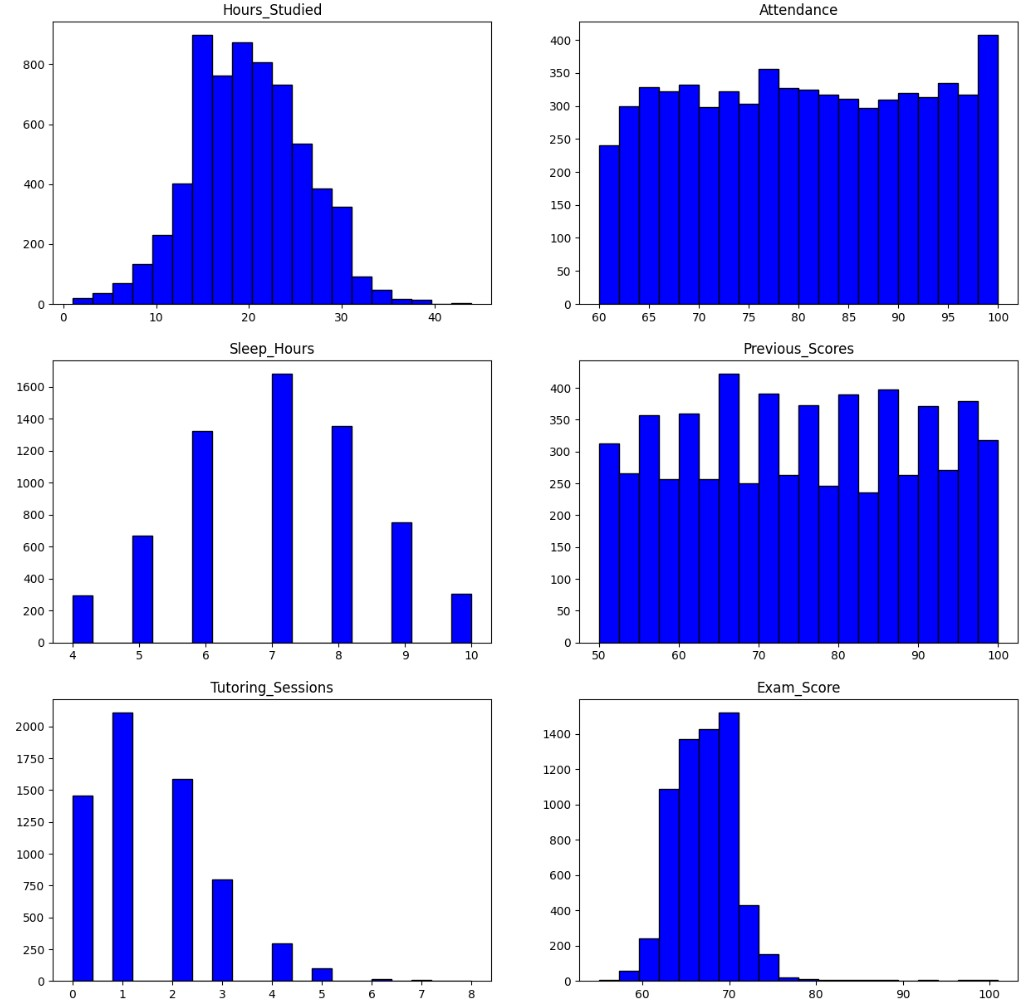
\includegraphics[width=0.9\textwidth]{./images/icon2.jpg}
    
\end{center}

Εύκολα μπορούμε να παρατηρήσουμε πως εφαρμόζουμε Standard Scaler στα χαρακτηριστικά Hours Studied και Sleep Hours αφού όπως μπορούμε να δούμε ακολουθούν κατά προσέγγιση κανονική κατανομή, MinMax Scaler στα χαρακτηριστικά Attendance και Previous Scores αφού προσεγγίζουν την ομοιόμορφη κατανομή και Robust Scaler στο χαρακτηριστικό Tutoring Sessions αφού όπως μπορούμε να δούμε περιέχει ακραίες τιμές. Η μεταβλητή στόχος Exam Scores δεν χρειάζεται να κλιμακωθεί αφού αποτελεί την εξαρτημένη μεταβλητή του μοντέλου μας.\\
\\
\noindent Οι σχέσεις για κάθε τύπο κλιμάκωσης δίνονται παρακάτω: 

\section*{Μέθοδοι Κλιμάκωσης}

\subsection*{StandardScaler}
Η μετατροπή με τη μέθοδο StandardScaler ορίζεται ως:
\[
X' = \frac{X - \mu}{\sigma}
\]
όπου:
\begin{itemize}
    \item \( X \): Η τιμή της παρατήρησης στο χαρακτηριστικό.
    \item \( \mu \): Ο μέσος όρος του χαρακτηριστικού.
    \item \( \sigma \): Η τυπική απόκλιση του χαρακτηριστικού.
\end{itemize}

\noindent Ο Standard Scaler μετασχηματίζει τα δεδομένα έτσι ώστε να έχουν μέση τιμή ίση με 0 και τυπική απόκλιση ίση με 1.

\subsection*{MinMaxScaler}
Η μετατροπή με τη μέθοδο MinMaxScaler ορίζεται ως:
\[
X' = \frac{X - X_{\text{min}}}{X_{\text{max}} - X_{\text{min}}}
\]
όπου:
\begin{itemize}
    \item \( X \): Η τιμή της παρατήρησης στο χαρακτηριστικό.
    \item \( X_{\text{min}} \): Η ελάχιστη τιμή του χαρακτηριστικού.
    \item \( X_{\text{max}} \): Η μέγιστη τιμή του χαρακτηριστικού.
\end{itemize}

\noindent Ο MinMax Scaler κλιμακώνει τα δεδομένα σε μια καθορισμένη περιοχή, συνήθως [0,1].



\subsection*{RobustScaler}
Η μετατροπή με τη μέθοδο RobustScaler ορίζεται ως:
\[
X' = \frac{X - Q_2}{Q_3 - Q_1}
\]
όπου:
\begin{itemize}
    \item \( X \): Η τιμή της παρατήρησης στο χαρακτηριστικό.
    \item \( Q_2 \): Η διάμεσος (median) του χαρακτηριστικού.
    \item \( Q_1 \): Το πρώτο τεταρτημόριο (25η εκατοστιαία θέση).
    \item \( Q_3 \): Το τρίτο τεταρτημόριο (75η εκατοστιαία θέση).\\
\end{itemize}

\noindent Ο Robust scaler μετασχηματίζει τα δεδομένα έτσι ώστε να έχουν κέντρο την διάμεσο η οποία γίνεται ίση με 0 και να μειώσει την επίδραση των ακραίων τιμών.\\

\noindent Γνωρίζουμε πως τα μοντέλα μηχανικής μάθησης δεν μπορούν να διαχειριστούν μη αριθμητικά δεδομένα. Επομένως, μέσω των encoders θα τα μετατρέψουμε με κατάλληλο τρόπο σε αριθμητικά χωρίς όμως να αλλάζουμε την κατηγορική τους ιδιότητα. Θα χρησιμοποιήσουμε Ordinal encoder για τα χαρακτηριστικά τα οποία περιέχουν κατηγορίες, οι οποίες έχουν κάποια φυσική σειρά(π.χ. "Low","Medium","High") και OneHot encoder για τα χαρακτηριστικά τα οποία περιέχουν κατηγορίες, οι οποίες δεν έχουν κάποια φυσική σειρά(π.χ. "Yes","No"). Επομένως τα κατηγορικά χαρακτηριστικά "Parental Involvement","Access to Resources","Motivation Level","Family Income", "Teacher Quality","Parental Education Level", "Distance from Home" και "Physical Activity" κωδικοποιούνται με ordinal encoding ενώ τα υπόλοιπα κατηγορικά χαρακτηριστικά με Onehot.

Η μέθοδος orindal encoding κωδικοποιεί με αριθμητικές τιμές κάθε κατηγορία με βάση την σειρά ή την θέση τους ξεκινώντας απο το 0. Για παράδειγμα εάν έχουμε τις κατηγορίες "Low","Medium","High" θα τους αναθέσει τις τιμές 0,1,2 αντίστοιχα. 

Η μέθοδος onehot encoding διαγράφει την κατηγορική στήλη και δημιουργεί για κάθε κατηγορία μια νέα που για κάθε παρατήρηση περιέχει την τιμή 1 αν το δείγμα ανήκει σε αυτήν την κατηγορία και 0 διαφορετικά. 
\subsection{Επιλογή χαρακτηριστικών}

Η επιλογή των χαρακτηριστικών που θα χρησιμοποιήσουμε για την πρόβλεψη του στόχου αποτελέι σημαντικό βήμα. Απο την μια προσπαθούμε να επιλέξουμε όλα τα σημαντικά χαρακτηριστικά έτσι ώστε να αποφύγουμε την υποπροσαρμογή, δηλαδή το μοντέλο μας να μην έχει τις απαραίτητες πληροφορίες για να αποτυπώσει την σχέση μεταξύ των δεδομένων και της μεταβλητής στόχου και απο την άλλη προσπαθούμε να επιλέξουμε όσο το δυνατό λιγότερα μη σημαντικά χαρακτηριστικά έτσι ώστε να αποφύγουμε την υπερπροσαρμογή, δηλαδή το μοντέλο μας να αποδίδει πολύ καλά στα δεδομένα εκπαίδευσης αλλά να αδυνατεί να γενικεύσει σε νέα δεδομένα.Αρχικά θα ορίσουμε 8 στο σύνολο μοντέλα παλινδρόμισης για τα οποία θα εξετάσουμε την απόδοση τους μέσω μιας μετρικής για κάθε συνδυασμό χαρακτηριστικών. Τα μοντέλα παλινδρόμισης τα οποία θα εξετάσουμε είναι τα εξής:\\
\begin{enumerate}
    \item Πολυωνιμικό μοντέλο παλινδρόμισης
    \item Γραμμική παλινδρόμιση
    \item Decision Tree παλινδρόμιση
    \item Random Forest παλινδρόμιση
    \item Support Vector παλινδρόμιση
    \item Gradient Boosting παλινδρόμιση
    \item Παλινδρόμιση Ridge
    \item Παλινδρόμιση Lasso\\
\end{enumerate}

 Για την πραγματοποίηση της παραπάνω διαδικασίας θα χρησιμοποιήσουμε τον αλγόριθμο Sequential feature selection (SFS). Θα μπορούσαμε να κάνουμε την διαδικασία αυτή και μέσω των πινάκων συσχέτισης Pearson, Cramer's V και ANOVA διαγράφοντας για κάθε ζεύγος μεταβλητών με ισχυρή συσχέτιση την μια απο τις δύο μεταβλητές αλλά με την διαφορά πως δεν θα είχαμε τόσο καλά αποτελέσματα όσο με την μέθοδο SFS. Η μέθοδος SFS με επιλογή για backwards selection ξεκινά με το πλήρες σύνολο χαρακτηριστικών. Το σύνολο εκπαίδευσης χωρίζεται σε k=cross-validation ίσα μέρη(folds). Σε κάθε επανάληψη, αφαιρείται ένα χαρακτηριστικό από το τρέχον σύνολο και το μοντέλο εκπαιδεύεται χρησιμοποιώντας τα εναπομείναντα χαρακτηριστικά. Το μοντέλο εκπαιδεύεται k φορές, χρησιμοποιώντας κάθε φορά ένα διαφορετικό fold ως σύνολο δοκιμής (test set), ενώ τα υπόλοιπα k-1 folds χρησιμοποιούνται ως σύνολο εκπαίδευσης (training set). Η απόδοση για κάθε αφαίρεση χαρακτηριστικού αξιολογείται με βάση τον μέσο όρο της απόδοσης για κάθε επιλογή fold ώς test set χρησιμοποιώντας κάποιο προκαθορισμένο κριτήριο, όπως το μέσο τετραγωνικό σφάλμα (MSE). Το χαρακτηριστικό που οδηγεί στη μικρότερη μείωση της απόδοσης αφαιρείται οριστικά από το σύνολο. Η διαδικασία συνεχίζεται μέχρι να επιτευχθεί ο επιθυμητός αριθμός χαρακτηριστικών. Για κάθε ένα απο τα μοντέλα παλινδρόμισης που αναφέραμε παραπάνω εντοπίσαμε τα χαρακτηριστικά τα οποία οδηγούν στο μικρότερο μέσο τετραγωνικό σφάλμα. Για την καλύτερη κατανόηση της μεθόδου, παρουσιάζεται παρακάτω η γραφική παράσταση του βέλτιστου αρνητικού μέσου τετραγωνικού σφάλματος. Η γραφική αφορά το μοντέλο παλινδρόμισης Decision Tree και βασίζεται στα χαρακτηριστικά που ελαχιστοποιούν το μέσο τετραγωνικό σφάλμα. Συγκεκριμένα, η γραφική απεικονίζει τη σχέση μεταξύ των χαρακτηριστικών όπως αυτά επιλέχθηκαν μέσω της συγκεκριμένης μεθόδου και του αρνητικού μέσου τετραγωνικού σφάλματος.

\begin{center}
    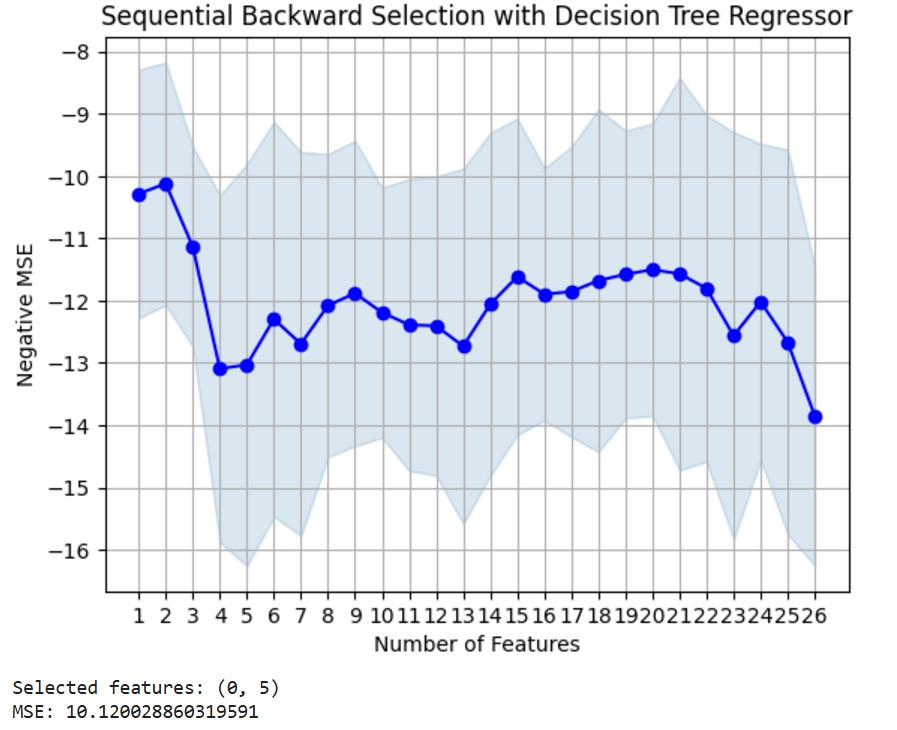
\includegraphics[width=0.9\textwidth]{./images/icon8.jpg}
    
\end{center}

Μπορούμε εύκολα να παρατηρήσουμε πως το το μεγαλύτερο αρνητικό μέσο τετραγωνικό σφάλμα επιτυγχάνετε για αριθμό χαρακτηριστικών ίσο με 2. Το αντίστοιχο καλύτερο μέσο τετραγωνικό σφάλμα είναι ίσο με $10.12$ και επιτυγχάνετε χρησιμοποιώντας την πρώτη και έκτη στήλη του πίνακα δεδομένων.

\subsection{Συσχέτιση των χαρακτηριστικών}
Η μελέτη της συσχέτισης μεταξύ των χαρακτηριστικών ενός dataset αποτελεί κρίσιμο βήμα στην κατανόηση της συμπεριφοράς των δεδομένων και στη διαδικασία επιλογής των κατάλληλων μεταβλητών για πρόβλεψη ή κατηγοριοποίηση. Μέσω της συσχέτισης, μπορούμε να εντοπίσουμε ποια χαρακτηριστικά σχετίζονται μεταξύ τους, ποια επηρεάζουν την ερμηνευτική μας μεταβλητή (target variable) και ποια είναι πιθανόν πλεονάζοντα ή αμελητέα.

Η παρούσα ανάλυση βασίζεται σε τρεις θερμόχαρτες (heatmaps) που απεικονίζουν τη σχέση μεταξύ διαφόρων αριθμητικών και κατηγορικών χαρακτηριστικών του δοθέντος dataset και μεταξύ κατηγορικών με αριθμητικών χαρακτηριστικών επίσης.

\begin{center}
    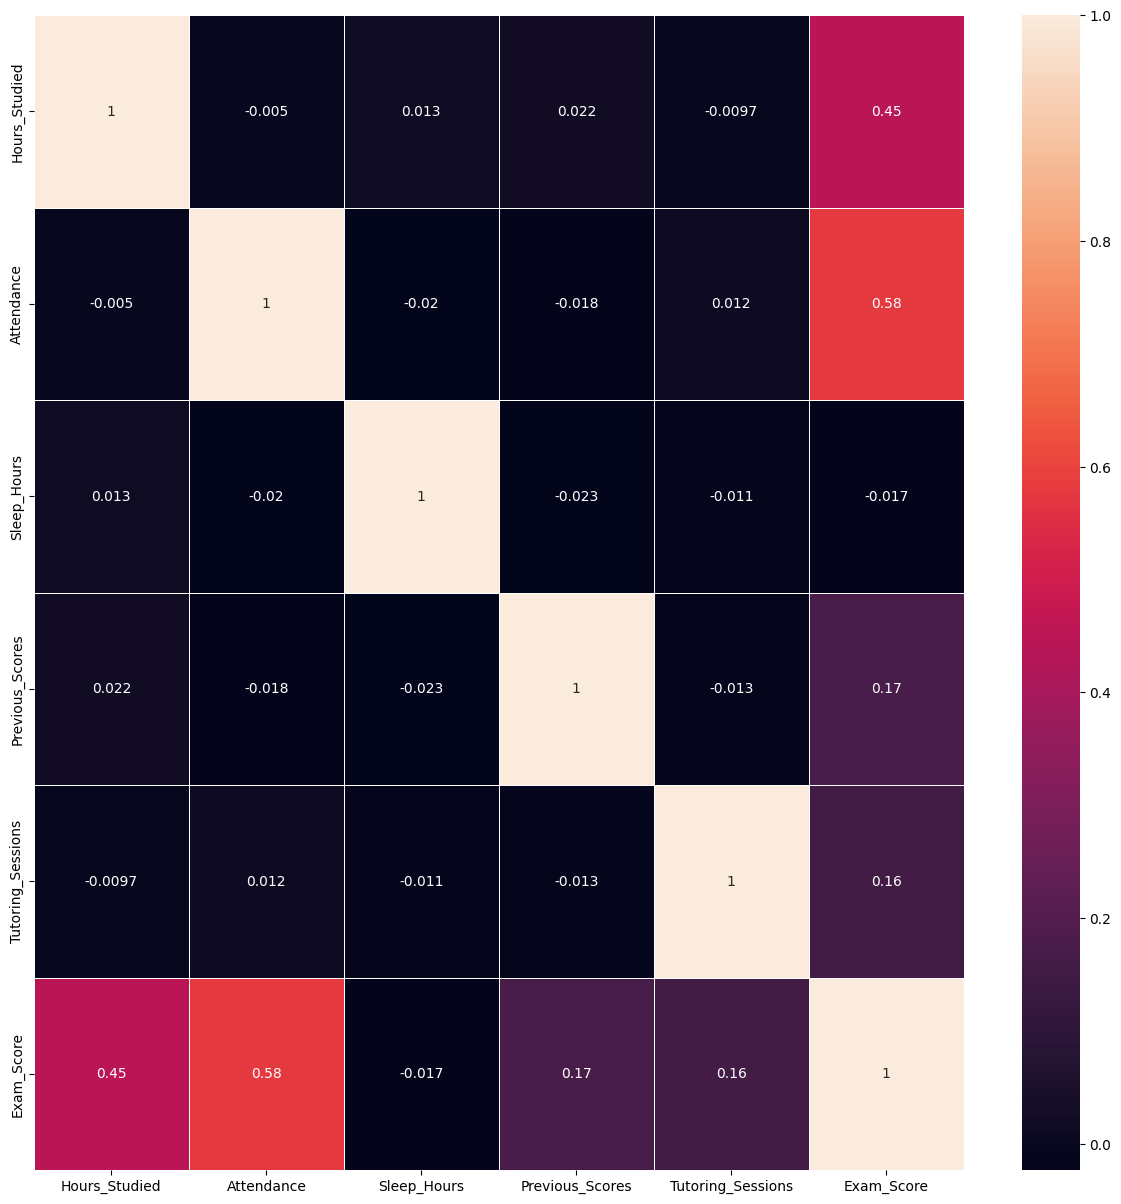
\includegraphics[width=0.9\textwidth]{./images/arithmetic_relation.png}
    
\end{center}

Στην παραπάνω εικόνα φαίνονται οι συσχετίσεις μεταξύ αριθμητικών μεταβλητών (Pearson correlation). Από την απιεκόνιση λοιπόν προκύπτει ότι:
\begin{itemize}
    \item Η \textbf{Παρουσία (Attendance)} έχει τη μεγαλύτερη συσχέτιση με τον \textbf{Τελικό Βαθμό (Exam_Score)}, με τιμή $0.58$, κάτι που δηλώνει ισχυρή θετική σχέση.
    \item Ακολουθεί η \textbf{Μελέτη (Hours_Studied)} με συσχέτιση $0.45$.
    \item Οι Previous_Scores, οι Tutoring_Sessions και οι Sleep_Hours έχουν χαμηλή έως αμελητέα συσχέτιση, δείχνοντας ότι δεν παίζουν σημαντικό ρόλο μεμονωμένα στη διαμόρφωση της τελικής επίδοσης.
\end{itemize}

Αυτό δείχνει πως η συνέπεια (μέσω παρουσιών) και η προσωπική μελέτη σχετίζονται άμεσα με την απόδοση του μαθητή.

Η επόμενη εικόνα παρουσιάζει τη μεταξύ τους σχέση των κατηγορικών μεταβλητών.

\begin{center}
    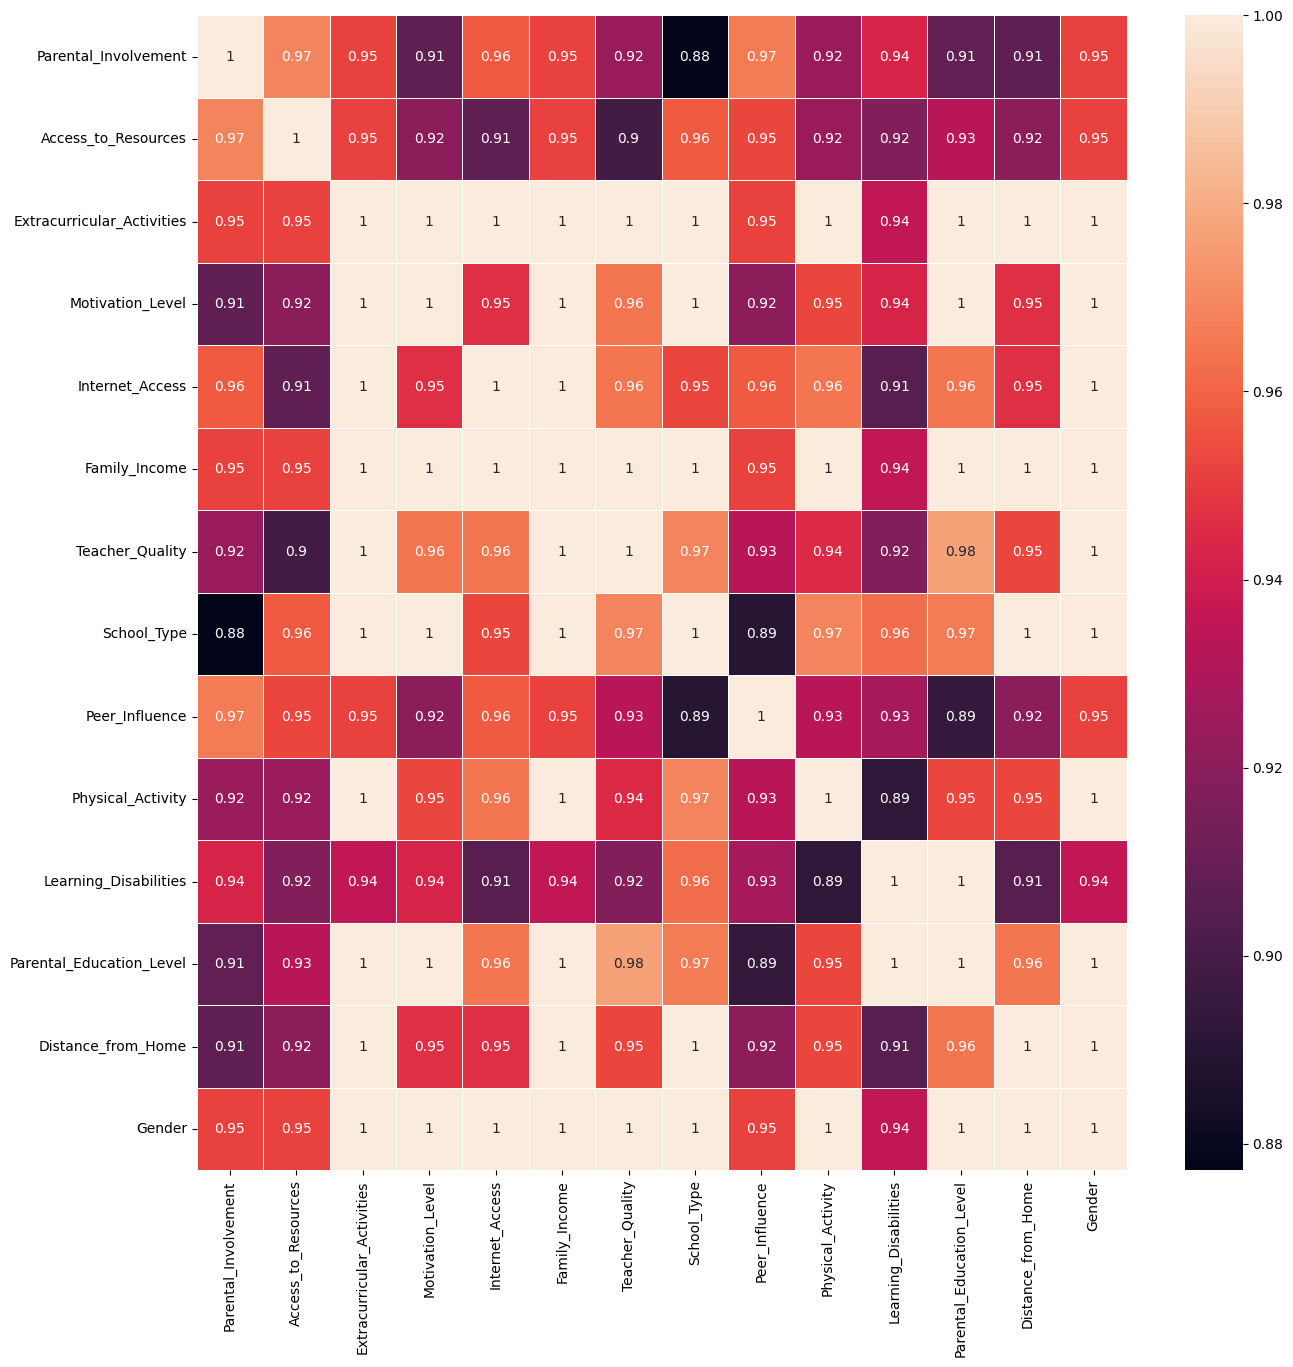
\includegraphics[width=0.9\textwidth]{./images/categorical_relation.png}
    
\end{center}

Η πλειονότητα των τιμών είναι εξαιρετικά υψηλές (άνω του $0.90$), γεγονός που υποδηλώνει:

\begin{itemize}
    \item Πολύ υψηλή συσχέτιση μεταξύ κοινωνικών, οικονομικών και οικογενειακών παραγόντων.
    \item Μεταβλητές όπως η Εκπαίδευση Γονέων, το Εισόδημα Οικογένειας, η Πρόσβαση σε Πόρους και η Ποιότητα Εκπαίδευσης είναι στενά συνδεδεμένες μεταξύ τους.
    \item Αυτό μπορεί να οδηγήσει σε πολυσυγγραμμικότητα (multicollinearity), που είναι σημαντικό να εντοπιστεί πριν τη χρήση μοντέλων πρόβλεψης ή παλινδρόμησης.
\end{itemize}

Η τρίτη και τελευταία εικόνα επεκτείνει την ανάλυση, εξετάζοντας πώς οι αριθμητικές μεταβλητές επηρεάζονται από κατηγορικές μεταβλητές όπως: Γονική Εμπλοκή, Πρόσβαση σε Πόρους, Ποιότητα Εκπαιδευτικού, Τύπος Σχολείου, Επίπεδο Εκπαίδευσης Γονέων, κ.ά.

\begin{center}
    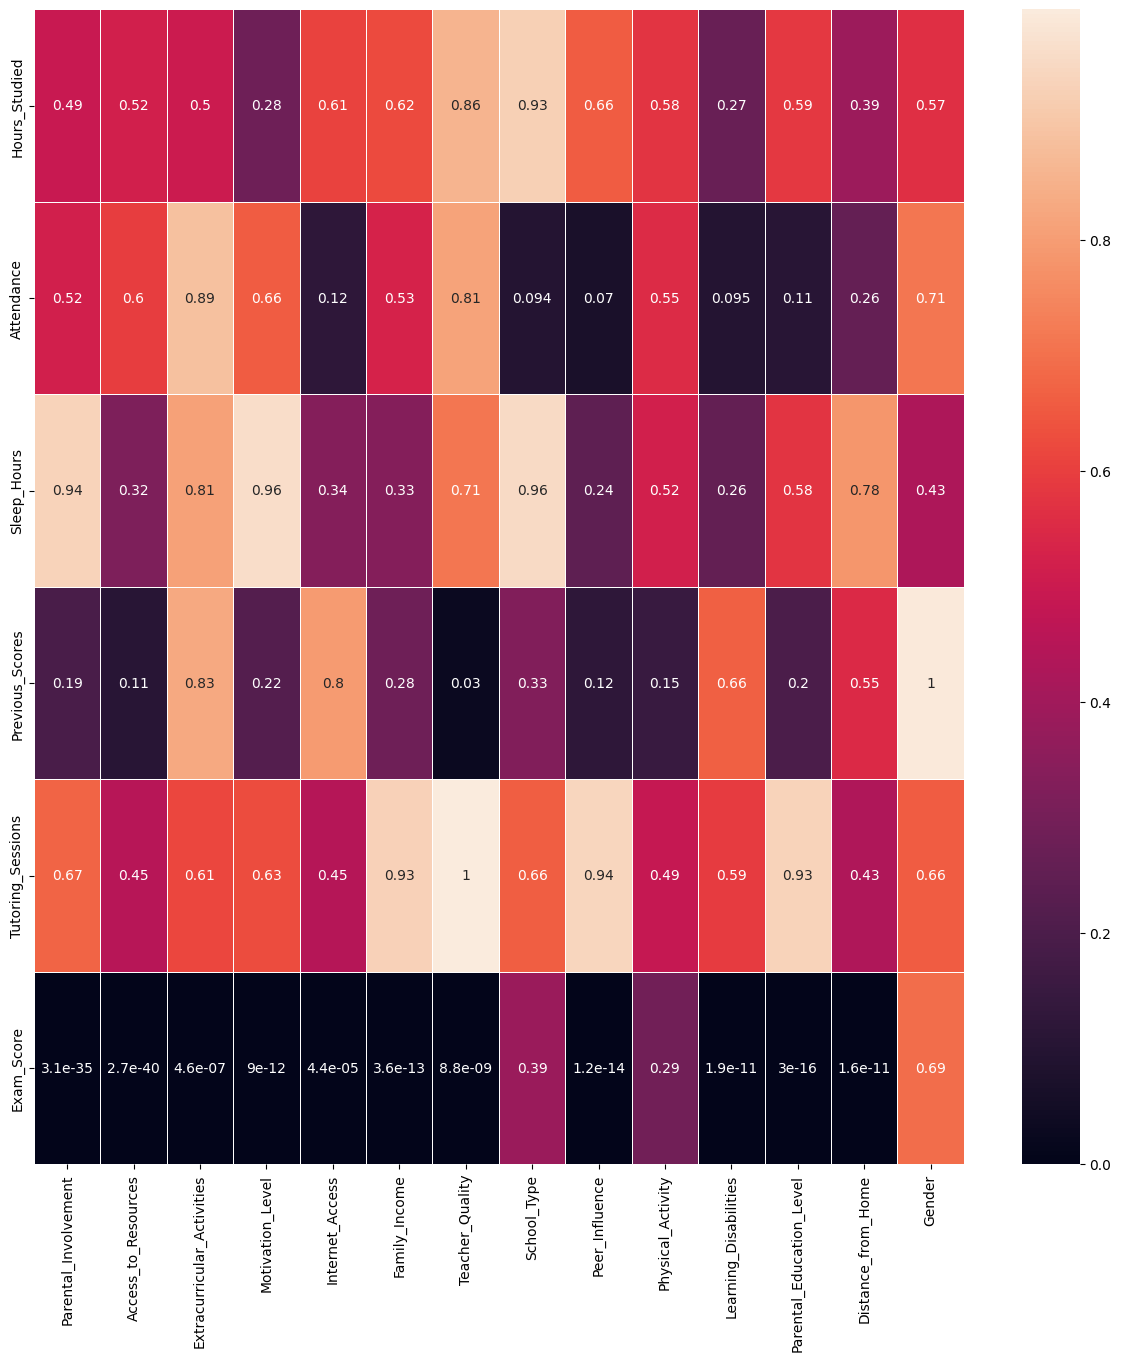
\includegraphics[width=0.9\textwidth]{./images/cat_arithmetic_rel.png}
    
\end{center}

Κάποιες ενδιαφέρουσες παρατηρήσεις:

\begin{itemize}
    \item Η \textbf{Γονική Εμπλοκή (Parental_Involvement)} και η \textbf{Ποιότητα Εκπαιδευτικού (Teacher_Quality)} έχουν υψηλή συσχέτιση με τις Φροντιστηριακές Συνεδρίες και τις Ώρες Μελέτης.
    \item Ο Τελικός Βαθμός φαίνεται να σχετίζεται στατιστικά σημαντικά με πολλές από τις κατηγορικές μεταβλητές, υποδεικνύοντας ότι παράγοντες όπως η οικογενειακή υποστήριξη, η πρόσβαση σε πόρους και το σχολικό περιβάλλον επηρεάζουν σημαντικά την απόδοση.
    \item Οι τιμές στον heatmap αντιπροσωπεύουν πιθανότητες (p-values), και τα πολύ μικρά νούμερα (π.χ. $1e-12$) δηλώνουν ισχυρή στατιστική συσχέτιση.
\end{itemize}

\subsection{Επιλογή υπερπαραμέτρων}
Για κάθε ένα από τα μοντέλα παλινδρόμησης που ορίσαμε παραπάνω, πραγματοποιήσαμε βελτιστοποίηση υπερπαραμέτρων (hyperparameter tuning) χρησιμοποιώντας τη μέθοδο GridSearchCV. Η βελτιστοποίηση έγινε για κάθε μοντέλο παλινδρόμισης χρησιμοποιώντας τα αντίστοιχα χαρακτηριστικά που επιλέχθηκαν ως βέλτιστα μέσω της μεθόδου Sequential Forward Selection (SFS). Στη διαδικασία, θέσαμε cross-validation = 10 και επιλέξαμε ως μετρική απόδοσης το μέσο τετραγωνικό σφάλμα(MSE). Η διαδικασία βελτιστοποίησης πραγματοποιήθηκε σε δύο στάδια. Aρχικά, εξετάσαμε ένα εύρος παραμέτρων γύρω από τις προεπιλεγμένες τιμές (default parameters), ώστε να αποκτήσουμε μια αρχική εικόνα για τη συμπεριφορά του μοντέλου. Στη συνέχεια, εστιάσαμε στις παραμέτρους που ανέδειξε η πρώτη διαδικασία ως πιο σημαντικές, προσαρμόζοντας το εύρος των τιμών τους για πιο λεπτομερή αναζήτηση. Με αυτόν τον τρόπο καταφέραμε να βελτιώσουμε περαιτέρω την απόδοση των μοντέλων μας, εξασφαλίζοντας καλύτερα αποτελέσματα.

Η μέθοδος GridSearchCV λειτουργεί ώς ακολούθως.
Το σύνολο εκπαίδευσης χωρίζεται σε k=cross-validation ίσα μέρη(folds). Στη συνέχεια, για κάθε συνδυασμό υπερπαραμέτρων που ορίζει ο χρήστης το μοντέλο εκπαιδεύεται k φορές, χρησιμοποιώντας κάθε φορά ένα διαφορετικό fold ως σύνολο δοκιμής (test set), ενώ τα υπόλοιπα k-1 folds χρησιμοποιούνται ως σύνολο εκπαίδευσης(training set). Η απόδοση κάθε συνδυασμού υπερπαραμέτρων αξιολογείται με βάση τον μέσο όρο της απόδοσης για κάθε επιλογή fold ώς test set. Τέλος, επιλέγεται ο συνδυασμός υπερπαραμέτρων που βελτιστοποιεί τη μετρική απόδοσης.
\subsection{Επιλογή μοντέλου}
Για να βρούμε το τελικό βέλτιστο μοντέλο παλινδρόμισης απο αυτά που εξετάσαμε κατασκευάσαμε το ραυδόγραμμα του μέσου τετραγωνικού σφάλματος για κάθε ένα απο τα μοντέλα παλινδρόμισης που βελτιστοποιήσαμε. Το ραυδόγραμμα αυτό παρουσιάζεται παρακάτω: 

\begin{center}
    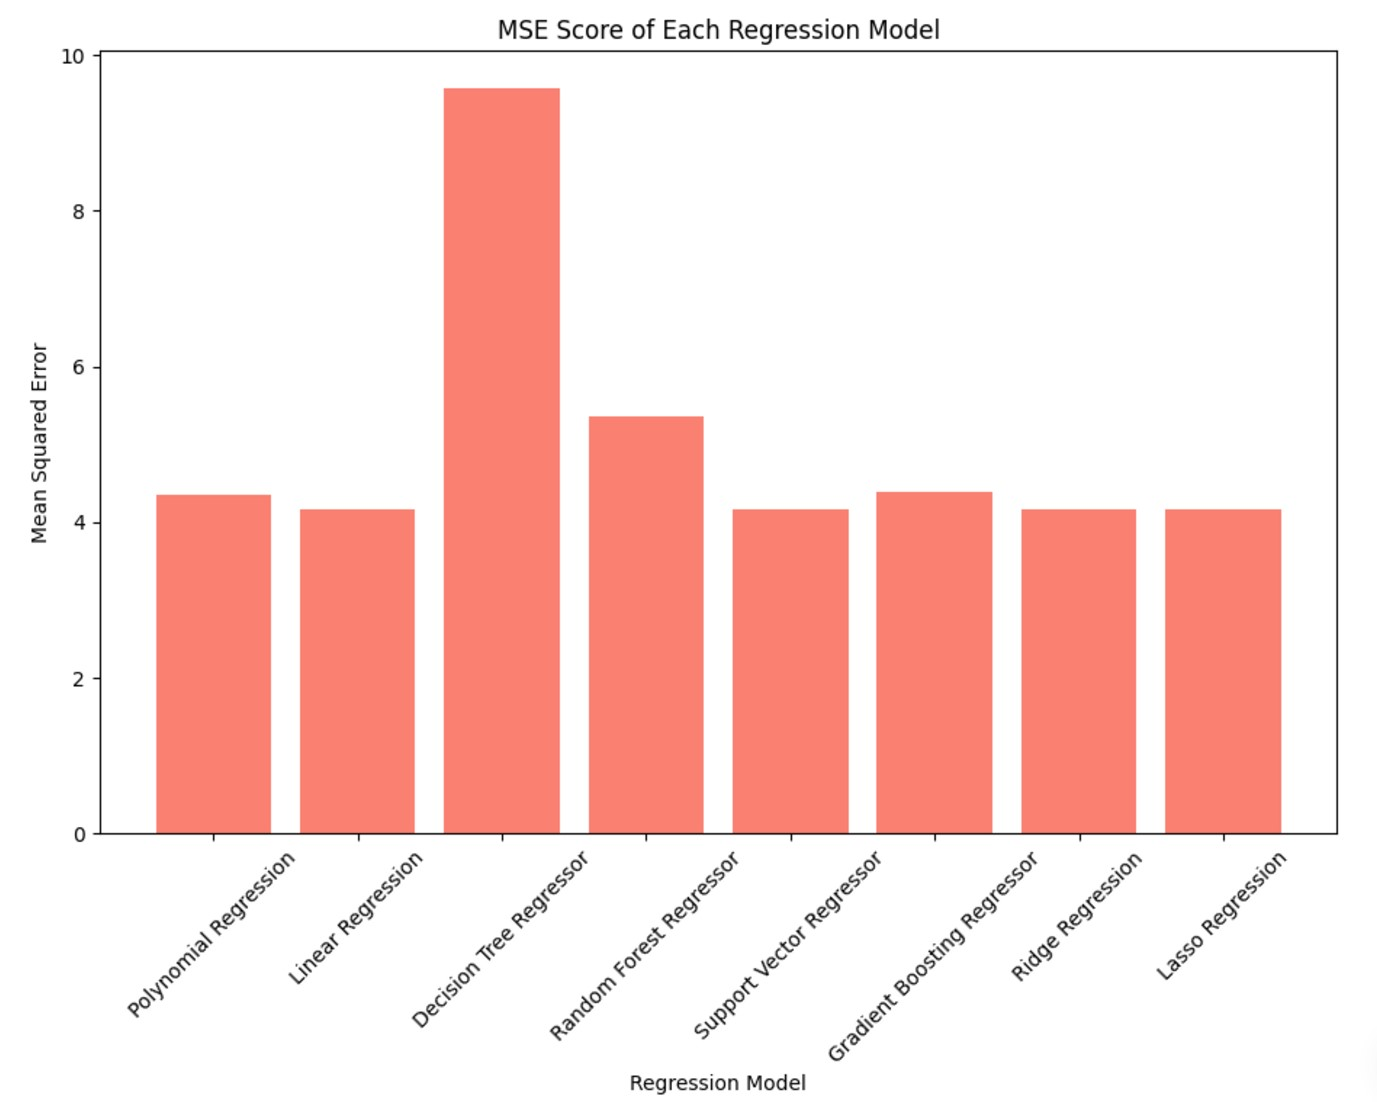
\includegraphics[width=0.9\textwidth]{./images/icon9.jpg}
    
\end{center}

Το μοντέλο το οποίο περιγράφει καλύτερα τα δεδομένα μας και προβλέπει σε καλύτερο βαθμό τον βαθμό του μαθητή με βάση την μετρική απόδοσης MSE είναι το μοντέλο παλινδρόμισης Lasso με μέσο τετραγωνικό σφάλμα ίσο με 4.155, επομένως έχουμε RMSE=\(\sqrt{MSE}=2.038\) και αυτό σημαίνει πως κατά μέσο όρο η πρόβλεψη μας για κάθε βαθμό εξέτασης διαφέρει κατά $2.038$ μονάδες απο την πραγματική τιμή. Με βάση την ανάλυση που κάναμε για τις υπερπαραμέτρους θέσαμε ρυθμό κανονικοποίησης (α) ίσο με 0.0001, μέγιστο αριθμό επαναλήψεων(max\_iter) ίσο με 500 και ανοχή σύγκλισης(tol) ίση με 0.1.Για να εξετάσουμε περαιτέρω την απόδοση του μοντέλου μας υπολογίσαμε τον συντελεστή προσδιορισμού \( R^2 \), ο οποίος ισούται με $0.733$  επομένως το μοντέλο μας εξηγά το 73.3\(\%\) της μεταβλητότητας του βαθμού του μαθητή(Exam Score). Τέλος, κατασκευάσαμε το γράφημα που φαίνετε παρακάτω όπου παρουσιάζει τις προβλεπόμενες τιμές του συνόλου δοκιμής σε σχέση με τις αντίστοιχες πραγματικές τιμές. 


\begin{center}
    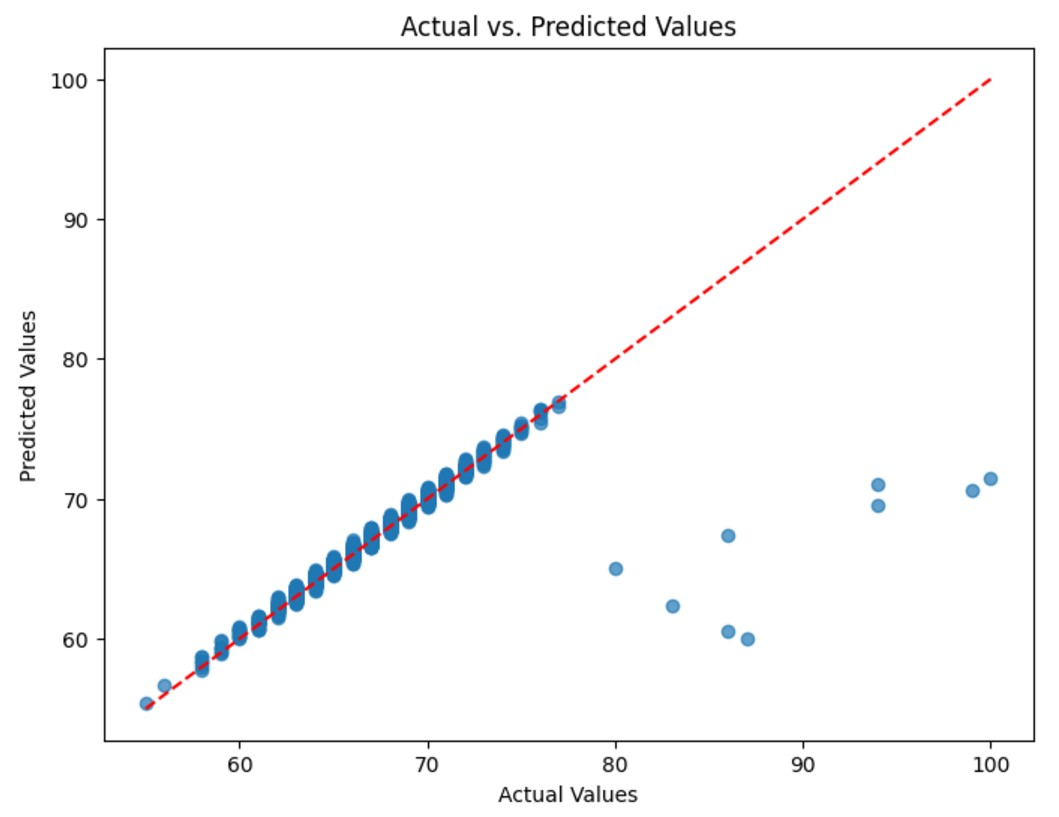
\includegraphics[width=0.89\textwidth]{./images/icon10.jpg}
    
\end{center}

Μπορούμε να παρατηρήσουμε πως το μοντέλο μας με βάση την παραπάνω γραφική παράσταση υπολογίζει σε αρκετά ικανοποιητικό βαθμό τον βαθμό του μαθητή για τιμές μικρότερες απο 80. Για τιμές μεγαλύτερες απο 80 δεν μπορούμε να πούμε το ίδιο. Αυτό οφείλετε στο ότι δεν υπάρχουν αρκετοί μαθητές οι οποίοι πήραν βαθμό μεγαλύτερο απο 80 στο training set (35 σε αριθμό), επομένως το μοντέλο μηχανικής μάθησης που δημιουργήσαμε δεν έχει αρκετά δεδομένα για να προβλέψει ικανοποιητικά τον τελικό βαθμό του μαθητή. Επίσης λόγω της μεγάλης διαφοράς στο πλήθος των δεδομένων στο training set για βαθμούς μικρότερους απο 80 σε σχέση με μεγαλύτερους απο αυτό, μπορεί να οδήγησε το μοντέλο μας σε υπερβολική εστίαση στα δεδομένα μικρότερα απο 80(biased ώς πρός αυτά τα δεδομένα) αφού τελικά θα οδηγούσε σε μικρότερο μέσο τετραγωνικό σφάλμα σε αντίθεση με το να το έκανε γενίκευση(generalize) και για τιμές μεγαλύτερες απο 80.

\newpage
\section{Το μοντέλο παλινδρόμισης Lasso}
\subsection{Εισαγωγή}

Η παλινδρόμιση $Lasso$ είναι μία παραλλαγή της γραμμικής παλινδρόμισης η οποία εισήχθη από τον $Tibshirani$ (1996). Εισάγει την κανονικοποίηση $l_1$ στο μέσο τετραγωνικό σφάλμα βοηθώντας με τον τρόπο αυτό το μοντέλο να επιλέγει χαρακτηριστικά που έχουν περισσότερη βαρύτητα στην προβλεπτική ικανότητα του μοντέλου έναντι άλλων. Το γεγονός αυτό είναι υψίστης σημασίας για δεδομένα υψηλών διαστάσεων (επεξηγηματικών μεταβλητών), αφού το μοντέλο γίνεται πιο αραιό \textlatin{sparsed} με αποτέλεσμα να μειώνεται κατά πολύ η υπολογιστική του πολυπλοκότητα διατηρώντας ωστόσο την επιθυμητή προβλεπτική ικανότητα.

\subsection{Λειτουργική Περιγραφή}
Η \textlatin{Lasso Regression} εισάγει την κανονικοποίηση $l_1$ ποινικοποιώντας τη συνάρτηση Μέσου Τετραγωνικού Σφάλματος με τον παράγοντα  $\lambda \sum_{i=1}^{p} |\beta_i|$.
\begin{equation}
    \hat{\beta}^{lasso} = \arg \min_{\beta} \left\{\sum_{i=1}^{N} \left( y_i - \beta_0 - \sum_{j=1}^{p} x_{ij} \beta_j \right)^2 + \lambda \sum_{j=1}^{p} |\beta_j| \right\}
\end{equation}
Ο όρος $\lambda \sum_{i=1}^{p} |\beta_i|$ "τιμωρεί τα μεγάλα βάρη των συντελεστών διότι αν επιτραπόυν συντελεστές με μεγάλη τιμή τότε η συνάρτηση κόστους αυξάνεται σημαντικά. Έτσι ο παράγοντας $\lambda$ μας δείχνει κατά πόσο θα ποινικοποιηθεί η τιμή των συντελεστών $\beta_i$ (δηλαδή κατά πόσο θα αυξηθεί η συνάρτηση κόστους)

\subsection{Μαθηματική Διατύπωση}
Δεδομένου ενός συνόλου δεδομένων με $n$ παρατηρήσεις και $p$ προβλεπτικές μεταβλητές, η παλινδρόμηση \textlatin{Lasso} ελαχιστοποιεί την ακόλουθη αντικειμενική συνάρτηση:
\begin{equation}
    \hat{\beta} = \arg \min_{\beta} \left\{ \sum_{i=1}^{n} (y_i - \sum_{j=1}^{p} X_{ij} \beta_j)^2 + \lambda \sum_{j=1}^{p} |\beta_j| \right\}
\end{equation}
όπου:
\begin{itemize}
    \item $y_i$ είναι οι πραγματικές τιμές-στόχοι,
    \item $X_{ij}$ είναι οι τιμές του χαρακτηριστικού $j$ στο δείγμα $i$,
    \item $\beta_j$ είναι οι συντελεστές που θέλουμε να εκτιμήσουμε,
    \item $\lambda$ είναι η παράμετρος ρύθμισης που ελέγχει την ένταση του περιορισμού.
\end{itemize}

\subsection{\textlatin{Coordinate Descent}}
Η μέθοδος \textlatin{Coordinate Lasso} είναι η πιο διαδεδομένη μέθοδος ελαχιστοποίησης της συνάρτησης κόστους για την παλινδρόμηση \textlatin{Lasso}. Η γνώστη βιβλιοθήκη \textlatin{scikit-learn} χρησιμοποιεί τη μέθοδο αυτή ως μέθοδο αυτή ως τεχνική εκπαίδευσης.\\
\vspace{0.1pt}\\

Η βασική του ιδέα  είναι, ότι δεν εστιάζει στην βελτιστοποίηση ταυτόχρονα όλων των συντελεστών $\beta_j$ του μοντέλου αλλά απομωνόνοντας έναν κάθε φορά, διατηρώντας όλους τους υπόλοιπους σταθερούς(επικεντρωνόμαστε δηλαδή στη μίνα δίασταση διατηρώντας τις υπόλοιπες σταθερές). Με τον τρόπο αυτό καταλήγουμε σε μία κλειστή έκφραση για τον υπολογισμό της εκτίμησης του κάθε συντελεστή.\\

Θα δούμε κάποιες στοιχειώδεις διαφορές ανάμεσα στον \textlatin{Coordinate Descent} και στον \textlatin{Gradient descent}:
\begin{itemize}
    \item \textbf{Η επιλογή βήματος}\\
    Ο \textlatin{Gradient descent} χρησιμοποιεί την παράμετρο $\beta$ που ορίζει πόσο μεγάλο θα είναι το βήμα του αλγορίθμου με σκοπό την προσέγγιση του ελαχίστου της συνάρτησης. Όμως η μη ορθή επιλογή του του βήματος μπορεί να οδηγήσει είτε σε αστάθεια(να μην προσεγγιστεί το ελάχιστο) είτε σε πολύ αργή σύγκλιση. Σε αντίθεση με τον \textlatin{Coordinate Descent} ο οποίος δεν χρειάζεται την παράμετρο $\beta$ για να λειτουργήσει αφού η ενημέρωση των συντελεστών γίνεται με β.
    \item \textbf{Μείωση Διαστατικότητας}\\
    Στον \textlatin{Gradient descent} δουλέύουμε με όλες τις διαστάσεις του προβλήματος, ενώ στον \textlatin{Coordinate Descent} διατηρούμε σταθερές όλες τις υπόλοιπες διαστάσεις και επικεντρωνόμαστε στην εκτίμηση ενός μόνο συντελεστή.
    \item\textbf{Απαίτηση Κυρτότητας}
    Ο \textlatin{Coordinate Descent} εγγυάται σύγκλιση σε ολικό ελάχιστο με την προϋπόθεση η συνάρτηση κόστους που ελαχιστοποιούμε να είναι της μορφής \[S(\beta) = f(\beta) + \sum_{j} h_j\beta_j\] και κυρτή. Εν αντιθέση με τον \textlatin{Gradient descent} ο οποίος δεν διαβεβαιώνει σύκγλιση σε ολικό ελάχιστο αλλά τοπικό. 
\end{itemize}

\subsection{\textlatin{Algorithm}}
Παρακάτω παρουσιάζεται ο βασικός ψευδοκώδικας:

% Προσθήκη στο preamble:
\SetAlgorithmName{Αλγόριθμος}{}{} % Ελληνικός τίτλος
\SetKwInput{KwData}{\textbf{Data:}} % Επεξεργασία KwData
\SetKwInput{KwResult}{\textbf{Result:}} % Επεξεργασία KwResult

\begin{algorithm}[H]
\caption{\textlatin{Lasso Regression με Coordinate Descent}}
\SetAlgoLined
\KwData{Design matrix \( \mathbf{X} \in \mathbb{R}^{n \times p} \), target vector \( \mathbf{y} \in \mathbb{R}^n \), regularization parameter \( \lambda \), max iterations \( T \), tolerance \( \epsilon \)} 
\KwResult{Coefficients \( \beta_0, \beta_1, ..., \beta_p \)}

\BlankLine
\textbf{Εκκίνηση:}\\
Ορίζουμε \( \beta_j^{(0)} = 0 \) για όλα τα \( j = 1,...,p \) \\
Υπολογίζουμε την αρχική σταθερά \( \beta_0 = \frac{1}{n} \sum_{i=1}^{n} y_i \) \\
\BlankLine

\textbf{Επανάληψη:} \\
\For{\( t = 1 \) \textbf{\textlatin{to}} \( T \)}{
    \For{\( j = 1 \) \textbf{\textlatin{to}} \( p \)}{
        Υπολογισμός μερικού υπολείμματος: \\
        \( r_j^{(t)} = \mathbf{y} - \beta_0^{(t)} - \sum_{k \neq j} \mathbf{X}_{:,k} \beta_k^{(t-1)} \) \\
        
        Ενημέρωση συντελεστή: \\
        \( z_j = \frac{1}{n} \mathbf{X}_{:,j}^\top r_j^{(t)} \) \\
        \( \beta_j^{(t)} = \mathcal{S}(z_j, \lambda) \) \quad \textlatin{(Soft-thresholding operator)} 
    }
    \BlankLine
    
    Έλεγχος σύγκλισης: \\
    \If{\( \|\beta^{(t)} - \beta^{(t-1)}\|_2 < \epsilon \)}{
        \textbf{Διακοπή επαναλήψεων}
    }
}
\BlankLine

\Return{\( \beta_0, \beta_1^{(T)}, ..., \beta_p^{(T)} \)} 
\end{algorithm}

\subsection{Κυρτότητα Συνάρτησης Κόστους}
Η κυρτότητα της συναρτησης κόστους προκύπτει από την κυρτότητα του μέσου τετραγωνικού σφάλματος, αφού είναι τετραγωνική συνάρτηση και η απόλυτη τιμή είναι επίσης κυρτή αλλά όχι διαφορίσιμη στο 0. Όπως ήδη γνωρίζουμε το άθροισμα κυρτών συναρτήσεων είναι κυρτή συνάρτηση, επομένως η συνάρτηση κόστους είναι κυρτή. Παρόλο που δεν είναι διαφορίσιμη στο 0 με την χρήση των υπερπαραγώγων επιτρέπεται η εύρεση βέλτιστων σημείων ακόμη και στα σημεία μη διαφορισιμότητας($\beta_j = 0$).


\subsection{\textlatin{Hyperparameters}}
Η βιβλιοθήκη \textlatin{scikit-learn} αποτελεί ένα από τα πιο δημοφιλή εργαλεία σε γλώσσα Python για την ανάπτυξη και εκπαίδευση μοντέλων μηχανικής μάθησης. Ανάμεσα στις μεθόδους παλινδρόμησης που παρέχει, ξεχωρίζει η \textlatin{Lasso}, η οποία προκειμένου να επιτύχει όχι μόνο βελτίωση της γενίκευσης \textlatin{(mitigation of overfitting)} αλλά και επιλογή χαρακτηριστικών \textlatin{(feature selection)} μέσω της προώθησης σπανιότητας στους συντελεστές, κάνει χρήση των υπερπαραμέτρων της. Επομένως, η απόδοση του μοντέλου \textlatin{Lasso} εξαρτάται σε μεγάλο βαθμό από την κατάλληλη ρύθμιση των \emph{υπερπαραμέτρων} (\textlatin{hyperparameters}). Η ορθή επιλογή τους μπορεί να βελτιστοποιήσει την ικανότητα γενίκευσης του μοντέλου, αποφεύγοντας τόσο την υπερπροσαρμογή \textlatin{(overfitting)} όσο και την υποπροσαρμογή \textlatin{(underfitting)}.

\begin{itemize}
    \item \textbf{\(\alpha\) (ή \(\lambda\))}: 
      Η πιο σημαντική παράμετρος που ελέγχει την ισχύ της \(\ell_1\) ποινής. 
      \[
        \min_{\beta_0,\beta}
        \left\{
          \frac{1}{2N}\sum_{i=1}^{N} \bigl(y_i - \beta_0 - \sum_{j=1}^{p} x_{ij}\beta_j \bigr)^2 
          \;+\;
          \alpha \sum_{j=1}^{p} |\beta_j|
        \right\}.
      \]
      \begin{itemize}
        \item Για \emph{μεγαλύτερη} τιμή \(\alpha\), ενισχύεται το φαινόμενο σπανιότητας, οδηγώντας σε περισσότερους μηδενικούς συντελεστές και πιθανή υποπροσαρμογή.
        \item Για \emph{μικρότερη} τιμή \(\alpha\), μειώνεται η πίεση προς μηδενισμό των συντελεστών, επιτρέποντας καλύτερη προσαρμογή, μα αυξάνοντας τον κίνδυνο υπερπροσαρμογής.
      \end{itemize}
    
    \item \textbf{\(\max\_iter\)}: 
      Ορίζει τον μέγιστο αριθμό επαναλήψεων του αλγορίθμου (\textlatin{Coordinate Descent}). Πολύ μικρή τιμή μπορεί να οδηγήσει σε μη ολοκληρωμένη σύγκλιση, ενώ πολύ μεγάλη τιμή επηρεάζει κυρίως τον χρόνο εκπαίδευσης.
    
    \item \textbf{\textlatin{tol}} \textlatin{(tolerance)}:
      Καθορίζει το κατώφλι κάτω από το οποίο οι αλλαγές στη συνάρτηση κόστους (ή στους συντελεστές) θεωρούνται αμελητέες, άρα ο αλγόριθμος σταματά. 
      \begin{itemize}
        \item Μικρό \(tol\) επιτρέπει βελτιστοποίηση ακριβείας, αυξάνοντας όμως τον χρόνο εκπαίδευσης.
        \item Μεγάλο \(tol\) επιταχύνει τη διαδικασία, αλλά ενδέχεται να αφήσει το μοντέλο σε υπο-βέλτιστη κατάσταση.
      \end{itemize}
    
    \item \textbf{\textlatin{fit\_intercept}}:
      Ενεργοποιεί ή απενεργοποιεί την εκτίμηση ανεξάρτητου όρου \(\beta_0\). Σε πολλές περιπτώσεις, η προεπιλογή \textlatin{True} είναι χρήσιμη, ιδίως όταν τα δεδομένα δεν είναι κεντραρισμένα.
    
    \item \textbf{\textlatin{normalize} ή προεπεξεργασία δεδομένων}:
      Σε παλαιότερες εκδόσεις του \textlatin{scikit-learn}, το \(normalize=True\) αναλάμβανε να κεντράρει και να κανονικοποιεί τα χαρακτηριστικά πριν από την εκπαίδευση. Για το $Lasso$, συνίσταται να κάνουμε \textlatin{\emph{manual}} \(standardization\), ώστε η \(\ell_1\) ποινή να εφαρμόζεται εξίσου σε όλες τις διαστάσεις.
    
    \item \textbf{\textlatin{selection}}:
      Επιλέγει τη στρατηγική με την οποία ενημερώνονται οι συντελεστές στον \textlatin{\emph{Coordinate Descent}}. 
      \begin{itemize}
        \item \textlatin{selection='cyclic'}: Η ενημέρωση γίνεται διαδοχικά για κάθε συντελεστή. Δηλαδή ξεκινάμε από το συντελεστή $\beta_1$, $\beta_2$ εώς ότου φτάσουμε στο συντελεστή $\beta_p$ από όπου ξανα αρχίζουμε από το $\beta_1$ με την ίδια σειρά iterate πάνω στους συντελεστές. 
        \item \textlatin{selection='random'}: Γίνεται τυχαία επιλογή συντελεστή κάθε φορά. Σε κάθε βήμα, επιλέγουμε τυχαία έναν από τους συντελεστές $\beta_j$ για ενημέρωση, αντί να ακολουθήσουμε μία προσυμφωνημένη σειρά 1,2,...,p. Αυτό σημαίνει ότι σε ορισμένες επαναλήψεις μπορεί να ενημερωθεί ο ίδιος συντελεστής διαδοχικά, ενώ άλλοι μπορεί να μείνουν αμετάβλητοι για κάποια βήματα, αναλόγως του \textlatin{random seed}.
      \end{itemize}
      Η τυχαία επιλογή, σε κάποιες περιπτώσεις, μπορεί να επιταχύνει τη σύγκλιση ή να βοηθήσει σε πιο πολύπλοκα προβλήματα.
    
    \end{itemize}

\newpage
\section{Σύγκριση με έρευνες}
\subsection{Επεξήγηση των παραμέτρων}
 Καταρχάς για να μπορούμε να κάνουμε την σύγκριση μεταξύ συγκεκριμένων ερευνών που υπάρχουν
 διαθέσιμες στο ευρύ κοινό και των αποτελεσμάτων που  προέκυψαν μέσω της δικής μας ανάλυσης,πρέπει
 πρώτα να κάνουμε μια ανάλυση της σχέσης μεταξύ του τελικού βαθμού του μαθητή και των διάφορων
 ανεξάρτητων μεταβλητών. \\
 
\noindent  Μέσω του μοντέλου μηχανικής μάθησης που δημιουργήσαμε πήραμε τα παρακάτω αποτελέσματα: \\

\begin{table}[ht]
\centering
\begin{tabular}{lrr}
\toprule
\textbf{Feature} & \textbf{Coefficient} \\
\midrule
Attendance                    & 7.945534e+00 \\
Previous\_Scores              & 2.432289e+00 \\
Tutoring\_Sessions            & 4.838539e-01 \\
Hours\_Studied                & 1.769307e+00 \\
Parental\_Involvement         & 1.006635e+00 \\
Access\_to\_Resources         & 1.021990e+00 \\
Motivation\_Level             & 5.513339e-01 \\
Family\_Income                & 5.666131e-01 \\
Teacher\_Quality              & 5.520568e-01 \\
Parental\_Education\_Level    & 4.946623e-01 \\
Distance\_from\_Home          & -4.593309e-01 \\
Physical\_Activity            & 1.992808e-01 \\
Extracurricular\_Activities\_No & -5.626076e-01 \\
Extracurricular\_Activities\_Yes & 1.337722e-16 \\
Internet\_Access\_No          & -8.974091e-01 \\
Peer\_Influence\_Negative     & -8.970209e-01 \\
Peer\_Influence\_Neutral      & -3.381165e-01 \\
Peer\_Influence\_Positive     & 1.176801e-01 \\
Learning\_Disabilities\_No    & 8.672434e-01 \\
\midrule
\textbf{Intercept} & \textbf{57.07844535052128} \\
\bottomrule
\end{tabular}
\label{tab:coefficients}
\end{table}

\noindent Εύκολα μπορούμε να συμπεράνουμε πως:\\

\begin{enumerate}
    \item \textbf{Parental Involvement} Ο βαθμός εμπλοκής των γονέων στην εκπαίδευση του μαθητή αναμένετε
 να συμβάλλει θετικά στον βαθμό του μαθητή. Συγκεκριμένα κατηγοριοποιείται σε τρία επίπεδα:
 ’Low’, ’Medium’ και ’High’. Για κάθε μεταβολή κατά ένα επίπεδο, από ’Low’ σε ’Medium’ ή
 από ’Medium’ σε ’High’, ο βαθμός του μαθητή αναμένετε να αυξηθεί κατά μία περίπου μονάδα.
 
 	\item \textbf{Access to Resources} Η πρόσβαση του μαθητή σε εκπαιδευτικό υλικό αναμένετε να συμβάλλει
 θετικά στον βαθμό του μαθητή. Συγκεκριμένα κατηγοριοποιείται σε τρία επίπεδα: ’Low’,’Medium’
 και ’High’. Για κάθε μεταβολή κατά ένα επίπεδο, από ’Low’ σε ’Medium’ ή από ’Medium’ σε
 ’High’, ο βαθμός του μαθητή αναμένετε να αυξηθεί κατά περίπου $1.02$ μονάδες.
 
 \item \textbf{Motivation Level} Το κίνητρο του μαθητή συμβάλλει αναμένετε να συμβάλλει θετικά στον βαθμό
 του μαθητή. Συγκεκριμένα κατηγοριοποιείται σε τρία επίπεδα: ’Low’, ’Medium’ και ’High’. Για
 κάθε μεταβολή κατά ένα επίπεδο, από ’Low’ σε ’Medium’ ή από ’Medium’ σε ’High’, ο βαθμός
 του μαθητή αναμένετε να αυξηθεί κατά περίπου $0.55$ μονάδες.
 
 \item \textbf{FamilyIncome} Το οικογενειακό εισόδημα του μαθητή αναμένετε νασυμβάλλει θετικά στον βαθμό
 του μαθητή. Συγκεκριμένα κατηγοριοποιείται σε τρία επίπεδα: ’Low’, ’Medium’ και ’High’. Για
 κάθε μεταβολή κατά ένα επίπεδο, από ’Low’ σε ’Medium’ ή από ’Medium’ σε ’High’, ο βαθμός
 του μαθητή αναμένετε να αυξηθεί κατά περίπου $0.57$ μονάδες.
 
 \item \textbf{Teacher Quality} Η εκπαιδευτική ικανότητα του καθηγητή του μαθητή αναμένετε να συμβάλλει
 θετικά στον βαθμό του μαθητή. Συγκεκριμένα κατηγοριοποιείται σε τρία επίπεδα: ’Low’,’Medium’
 και ’High’. Για κάθε μεταβολή κατά ένα επίπεδο, από ’Low’ σε ’Medium’ ή από ’Medium’ σε
 ’High’, ο βαθμός του μαθητή αναμένετε να αυξηθεί κατά περίπου $0.55$ μονάδες.
 
 \item \textbf{Parental Education Level} Το επίπεδο εκπαίδευσης του γονέα του μαθητή αναμένετε να συμβάλλει
 θετικά στον βαθμό του μαθητή. Συγκεκριμένα κατηγοριοποιείται σε 3 επίπεδα: ’High School’,
 ’College’ και ’Postgraduate’. Για κάθε μεταβολή κατά ένα επίπεδο, από ’High School’ σε ’Col
lege’ ή από ’College’ σε ’Postgraduate’, ο βαθμός του μαθητή αναμένετε να αυξηθεί κατά περίπου
 $0.49$ μονάδες.
 
 \item \textbf{Distance from Home} Η απόσταση του σχολείου απο το σπίτι του μαθητή αναμένετε να συμβάλλει
 αρνητικά στον βαθμό του μαθητή. Συγκεκριμένα κατηγοριοποιείται σε τρία επίπεδα: ’Near’,
 ’Moderate’ και ’Far’. Για κάθε μεταβολή κατά ένα επίπεδο, από ’Near’ σε ’Moderate’ ή από
 ’Moderate’ σε ’Far’, ο βαθμός του μαθητή αναμένετε να μειωθεί κατά περίπου $0.46$ μονάδες.
 
 \item \textbf{Physical Activity} Το επίπεδο φυσικής δραστηριότητας του μαθητή αναμένετε να συμβάλλει θετικά
 στον βαθμό του μαθητή. Συγκεκριμένα κατηγοριοποιείται σε 7 επίπεδα: ’Sedentary’, ’Light’,
 ’Moderate’, ’Active’, ’Very Active’, ’Highly Active’ και ’Athlete’. Για κάθε μεταβολή κατά ένα
 επίπεδο, από ’Sedentary’ σε ’Light’, από ’Light’ σε ’Moderate’ κ.ο.κ. , ο βαθμός του μαθητή
 αναμένετε να αυξηθεί κατά περίπου $0.2$ μονάδες.

 \item \textbf{Peer Influence}  Η μορφή της επιρρόης που δέχεται ο μαθητής απο ομήλικους του επιρεάζει και
 τον βαθμό του. Συγκεκριμένα η επιρροή αυτή χωρίζετε σε 3 κατηγορίες ’Negative’, ’Neutral’ και
 ’Positive’. Για μεταβολή αυτού απο ’Negative’ σε ’Neutral’, ο βαθμός του μαθητή αναμένετε να
 αυξηθεί κατά περίπου $0.56$ μονάδες. Για μεταβολή αυτού απο ’Neutral’ σε ’Positive’, ο βαθμός
 του μαθητή αναμένετε να αυξηθεί κατά περίπου $0.46$ μονάδες.
    
    \item \textbf{Extracurricular Activities}  Η συμμετοχή του μαθητή σε εξωσχολικές δραστηριότητες αναμένετε
 να συμβάλλει θετικά στον βαθμό του μαθητή. Συγκεκριμένα εάν ο μαθητής συμμετέχει σε εξωσχολικές
 δραστηριότητες ο βαθμός του αναμένετε να αυξηθεί κατά περίπου $0.56$ μονάδες.
 
 \item \textbf{Internet Access}  Η πρόσβαση του μαθητή στο διαδύκτιο αναμένετε να συμβάλλει θετικά στον
 βαθμό του μαθητή. Συγκεκριμένα εάν ο μαθητής έχει πρόσβαση στο διαδίκτυο ο βαθμός του
 αναμένετε να αυξηθεί κατά περίπου $0.90$ μονάδες.
 
 \item \textbf{Learning Disabilities} Η ύπαρξη μαθησιακών δυσκολιών στον μαθητή αναμένετε να συμβάλλει
 αρνητικά στον βαθμό του. Συγκεκριμένα εάν ο μαθητής έχει μαθησιακές δυσκολίες ο βαθμός του
 αναμένετε να μειωθεί κατά περίπου $0.87$ μονάδες.\\
\end{enumerate}

\noindent Η επεξήγηση των μεταβολών για κάθε χαρακτηριστικό το οποίο παίρνει αριθμητικές τιμές θέλει
 προσοχή. Αυτό οφείλετε στο ότι τα βάρη που υπολογίσαμε δείχνουν την μεταβολή του βαθμού του
 μαθητή όχι για τις μεταβλητές Attendance, Previous Scores , Tutoring Sessions και Hours Studied
 αλλά για τις κλιμακωμένες τιμές τους. Για να βρούμε την πραγματική τους σχέση θα κινηθούμε
 ώς ακολούθως:\\
 
 \begin{itemize}
    \item Εάν το χαρακτηριστικό κλιμακώθηκε μέσω Standard Scaler(Συγκεκριμένα η Hours Studied) ,τότε για κάθε μεταβολή κατά μια μονάδα του χαρακτηριστικού αυτού θα έχουμε μεταβολή του βαθμού του μαθητή κατά coeff/std(feature) μονάδες, όπου coeff η αντίστοιχη τιμή του coefficient του χαρακτηριστικού όπως φαίνετε στον πίνακα παραπάνω και std(feature) η τυπική του απόκλιση που προκύπτει απο τα δεδομένα.
    
    \item Εάν το χαρακτηριστικό κλιμακώθηκε μέσω MinMax Scaler(Συγκεκριμένα οι Attendance και Previous Scores) ,τότε για κάθε μεταβολή κατά μια μονάδα του χαρακτηριστικού αυτού θα έχουμε μεταβολή του βαθμού του μαθητή κατά coeff/(max(feature)-min(feature)) μονάδες, όπου coeff η αντίστοιχη τιμή του coefficient του χαρακτηριστικού όπως φαίνετε στον πίνακα παραπάνω, min(feature) η ελάχιστη τιμή του χαρακτηριστικού αυτού στα δεδομένα και max(feature) η μέγιστη τιμή του χαρακτηριστικού στα δεδομένα.
    
     \item Εάν το χαρακτηριστικό κλιμακώθηκε μέσω Robust Scaler(Συγκεκριμένα η Tutoring Sessions) ,τότε για κάθε μεταβολή κατά μια μονάδα του χαρακτηριστικού αυτού θα έχουμε μεταβολή του βαθμού του μαθητή κατά coeff/IQR(feature) μονάδες, όπου coeff η αντίστοιχη τιμή του coefficient του χαρακτηριστικού όπως φαίνετε στον πίνακα παραπάνω και IQR(feature) το ενδοτεταρτημοριακό του εύρος που προκύπτει απο τα δεδομένα.
  \end{itemize}
  
\noindent Μέσω της ανάλυσης που κάναμε πήραμε τα παρακάτω διαγράμματα που δείχνουν την σχέση μεταξύ των ποσοτικών χαρακτηριστικών και του βαθμού του μαθητή: \\

\begin{center}
    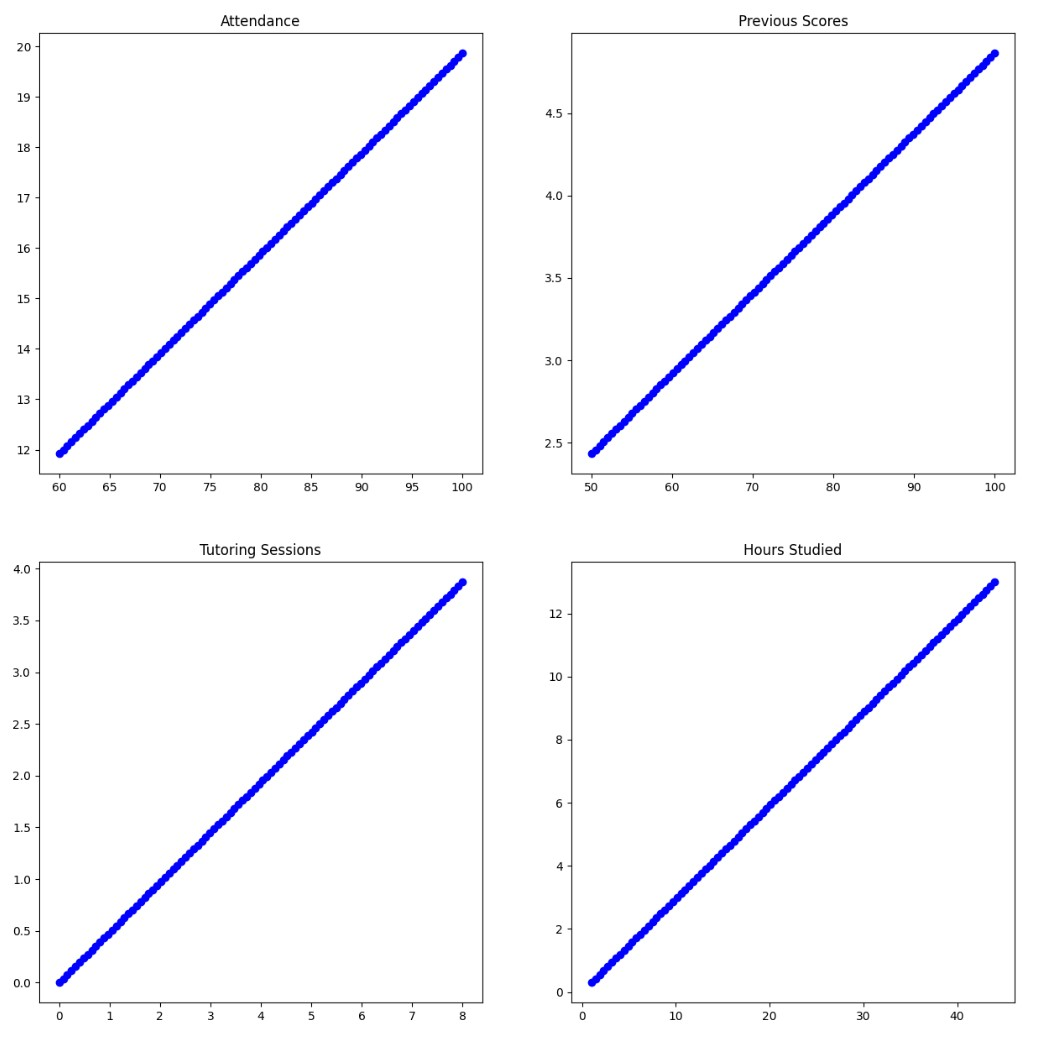
\includegraphics[width=0.89\textwidth]{./images/icon12.jpg}
    
\end{center}

Εύκολα μπορούμε να συμπεράνουμε πως: \\

\begin{enumerate}
    \item \textbf{Attendance} Το ποσοστό της προσέλευση του μαθητή στο μάθημα αναμένετε
 να συμβάλλει στον προσδιορισμό του βαθμού του μαθητή. Συγκεκριμένα η μεταβολή κατά μια μονάδα του χαρακτηριστικού αυτού αναμένετε να μεταβάλλει τον βαθμό του μαθητή κατά περίπου $0.2$ μονάδες.
 
 	\item \textbf{Previous Scores} Ο μέσος όρος των βαθμών του μαθητή απο προηγούμενες εξετάσεις αναμένετε
 να συμβάλλει στον προσδιορισμό του βαθμού του μαθητή. Συγκεκριμένα η μεταβολή κατά μια μονάδα του χαρακτηριστικού αυτού αναμένετε να μεταβάλλει τον βαθμό του μαθητή κατά περίπου $0.05$ μονάδες.
 
 \item \textbf{Tutoring Sessions} Ο αριθμός των φροντιστηριακών μαθημάτων ανά μήνα του μαθητή αναμένετε
 να συμβάλλει στον προσδιορισμό του βαθμού του μαθητή. Συγκεκριμένα η μεταβολή κατά μια μονάδα του χαρακτηριστικού αυτού αναμένετε να μεταβάλλει τον βαθμό του μαθητή κατά περίπου $0.48$ μονάδες.
 
 \item \textbf{Hours Studied} Ο αριθμός των ωρών που διάβασε ο μαθητής μέσα στην βδομάδα αναμένετε
 να συμβάλλει στον προσδιορισμό του βαθμού του μαθητή. Συγκεκριμένα η μεταβολή κατά μια μονάδα του χαρακτηριστικού αυτού αναμένετε να μεταβάλλει τον βαθμό του μαθητή κατά περίπου $0.29$ μονάδες.
 
\end{enumerate}
 
Στο μοντέλο μηχανικής μάθησης που προσαρμόσαμε για την εκτίμηση της ακαδημαϊκής επίδοσης των μαθητών 
με βάση ορισμένα χαρακτηριστικά τους, οι σημαντικότεροι προβλεπτικοί παράγοντες που προέκυψαν ήταν:\\

\begin{enumerate}

  \item Attendance (Φοίτηση/Παρουσίες)
  
  \item Previous\_{Scores} (Προηγούμενες Επιδόσεις)
  
  \item Tutoring\_{Sessions} (Πρόσθετη Διδακτική Στήριξη/Φροντιστηριακά μαθήματα)
  
  \item Hours\_{Studied} (Ώρες Μελέτης)
  
  \item Parental\_{Involvement} (Γονεϊκή Εμπλοκή)
  
  \item Access\_{to}\_{Resources} (Πρόσβαση σε Πηγές/Υλικό)
  
  \item Motivation\_{Level} (Επίπεδο Κινήτρων)
  
  \item Family\_{Income} (Οικογενειακό Εισόδημα)
  
  \item Teacher\_{Quality} (Ποιότητα Διδασκαλίας/Εκπαιδευτικών)
  
  \item Parental\_{Education}\_{Level} (Εκπαιδευτικό Επίπεδο Γονέων)
  
  \item Distance\_{from}\_{Home} (Απόσταση από το Σπίτι)
  
  \item Physical\_{Activity} (Σωματική Άσκηση)
  
  \item Extracurricular\_{Activities} (Συμμετοχή σε Εξωσχολικές Δραστηριότητες)
  
  \item Internet\_{Access} (Πρόσβαση στο Διαδίκτυο)
  
  \item Peer\_{Influence} (Επιρροή Ομηλίκων)
  
  \item Learning\_{Disabilities} (Μαθησιακές Δυσκολίες)
  
\end{enumerate}

Παρακάτω θα παραθέσουμε σύγκριση της σημαντικότητας των παραγόντων αυτών με ερέυνες που έχουν πραγματοποιηθεί 
πάνω στην επίδοση των μαθητών.\\

\begin{itemize}
\item \textbf{Learning\_{Disabilities}\_{No}}\\
Η παρουσία μαθησιακών δυσκολιών στους μαθητές είναι ένας από τους παράγοντες που επηρεάζουν την ακαδημαϊκή τους επίδοση. Αρκετά φανερό το γιατί επηρεάζεται αλλά θα διεισδύσουμε λίγο παραπάνω στο γιατί.
Αρχικά το χαρακτηριστικό αυτό υποδηλώνει την απουσία μαθησιακών δυσκολιών στους μαθητές, με αποτέλεσμα να πετυχαίνουν σίγουρα πιο υψηλές βαθμολογίες έναντι εκείνων που αντιμετωπίζουν τέτοια προβληματα.
Παρόλα αυτά δεν αντικατοπτρίζει χαμηλότερη νοημοσύνη έναντι των υπολοίπων μαθητών η ύπαρξη μαθησιακών δυσκολιών, αλλά υποδηλώνει μια διαφορετική προσέγγιση στη μάθηση. 
Με την κατάλληλη υποστήριξη, προσαρμοσμένες εκπαιδευτικές μεθόδους, και την έγκαιρη ανίχνευση των δυσκολιών, οι μαθητές μπορούν να αξιοποιήσουν πλήρως τις δυνατότητές τους. 
Ο ρόλος του σχολείου και των ειδικών στη σωστή διάγνωση είναι αποφασιστικός για την υποστήριξη αυτών των παιδιών. Με βάση την πηγή επισημαίνεται πως οι αδιάγνωστες μαθησιακές δυσκολίες οδηγούν σε 
χαμηλότερη απόδοση, ενώ η έγκαιρη διάγνωση βοηθά στην κατάλληλη παιδαγωγική παρέμβαση.

\item \textbf{Attendance}\\
Η παρουσια των μαθητών στους χώρους της σχολικής τάξης είναι υψίστης σημασίας, όπως άλλοστε έδειξε και 
το μοντέλο μας αφού ο συντελεστής του Attendance ήταν ο δεύτερος μεγαλύτερος με βάση το μοντέλο παλινδρόμησης Lasso. 
Το γεγονός αυτό υποδυκνύει ότι η τακτική παρουσία στο σχολείο είναι ισχυρά συσχετισμένη με την τελική επίδοση.
Σύμφωνα με τις πηγές η συστηματική παρακολούθηση βοηθάει τους μαθητές να κατανοήσουν σε μεγαλύτερο βάθος,
την ύλη που διδάσκονται λόγω της συνεχόμενης ροής και συνοχής της γνώσης που λαμβάνουν. Από την άλλη πλευρά,
οι μαθητές που δεν παρεβρίσκονται στην τάξη αδυνατούν να καλύψουν τα κενά, με προφανείς συνέπειες στους βαθμούς τους.
Αυτό έρχεται σε πλήρη συμφωνία με το δικό μας αποτέλεσμα. Μάλιστα, σε έρευνες που επικαλείται η ίδια πηγή, 
οι επιδόσεις των μαθητών αυξάνονται αναλογικά με το ποσοστό παρακολούθησης δηλαδή η σχέση των απουσιών
και του μέσου όρου των μαθητών είναι αντιστρόφος ανάλογη (ελάχιστες απουσίες – υψηλότερος μέσος όρος).

\item \textbf{Family\_{Income}}\\
Το οικονομικό υπόβαθρο της οικογένειας επηρεάζει την εκπαιδευτική πορεία του μαθητή, κυρίως μέσω της δυνατότητας 
για επιπρόσθετη εκπαιδευτική υποστήριξη, όπως φροντιστηριακά μαθήματα ή αγορές βιβλίων και τεχνολογικού εξοπλισμού τα οποία όχι απλώς 
επιταχύνουν τη διαδικασία της μάθησης αλλά παράλληλα την καθιστούν και πιο ευχάριστη. 
Για το λόγο αυτό παρατηρούμε και το ποσοστό του 95\%  θετικής συσχέτισης του με το Access\_{to}\_{Resources}.
Παράλληλα, σε οικογένειες με περιορισμένο εισόδημα, η πρόσθετη πίεση για βιοπορισμό μπορεί να επηρεάσει έμμεσα τη σχολική προετοιμασία και τη διαθεσιμότητα χρόνου για μελέτη.

\item \textbf{Teacher\_{Quality}}\\
Με υψηλό συντελεστή παρατηρήσαμε και τον παράγοντα της ποιότητας των δασκάλων. Οι διδακτικές πρακτικές διαδραματίζου σημαντικό ρολο στη βελτίωση
των επιδόσεων των μαθητών.Η αποτελεσματική διδασκαλία συνδέεται άμεσα με την εδραίωση ενθουσιασμού στους μαθητές και την καλύτερη κατανόηση της ύλης. Ένας καταρτισμένος 
και ευαισθητοποιημένος εκπαιδευτικός μπορεί να απλοποιήσει πολύπλοκες έννοιες, να κινητοποιήσει τους μαθητές και να ενθαρρύνει την ενεργητική συμμετοχή. Όταν η διδακτική
προσέγγιση προσαρμόζεται στις εκπαιδευτικές ανάγκες κάθε τάξης, οι επιδόσεις βελτιώνονται ουσιαστικά. Το γεγονός ότι ο συντελεστής στο μοντέλο δεν είναι πολύ μεγάλος ίσως 
εξηγείται από το γεγονός ότι η «ποιότητα εκπαιδευτικών» πολλές φορές επηρεάζεται από υποκειμενικές αντιλήψεις των μαθητών ή και από δομικές συνθήκες του σχολείου.

\item \textbf{Motivation\_{Level}}\\
Το Motivation\_{Level} με συντελεστή $5.51$ υποδυκνύει ότι οι μαθητές με έντονα εσωτερικά ή εξωτερικά κίνητρα σημειώνουν υψηλότερες επιδόσεις. Τα κίνητρα μαθητών ποικίλλουν με 
βάση την αυτοπεποίθηση, τις φιλοδοξίες και το ενδιαφέρον τους για το μάθημα. Ένας μαθητής με υψηλό επίπεδο κινήτρων τείνει να αφιερώνει περισσότερο χρόνο στη μελέτη, να 
αναζητά επιπλέον υλικό και να συμμετέχει ενεργά στην τάξη. Η ψυχολογική αυτή διάσταση είναι καθοριστική, καθώς μπορεί να ξεπεράσει ακόμη και δυσκολίες στην πρόσβαση σε 
πόρους, επιδρώντας θετικά στη γενικότερη ακαδημαϊκή εικόνα. Αυτό επιβεβειώνεται και από την πηγή που αναφέρεται στην υποεπίδοση και την αυτορύθμιση  τονίζεται η σημασία 
του κινήτρου και της αυτορρύθμισης (self-regulation) στην επίτευξη στόχων. Συνεπώς, η ένδειξη ότι το επίπεδο κινήτρων έχει τόσο ισχυρό αντίκτυπο εναρμονίζεται με τη διεθνή βιβλιογραφία.

\item \textbf{Tutoring\_{Sessions}}\\
Η φροντιστηριακή Υποστήριξη (Tutoring\_{Sessions}) έχει επίσης σημαντικό συντελεστή στο μοντέλο μας. Σύμφωνα με τις έρευνες, η επιπρόσθετη διδακτική υποστήριξη(ιδιάιτερα ή φροντιστήρια) 
λειτουργεί θετικά κυρίως σε μαθητές με ελλείψεις, καθώς οι μικρές ομάδες ή τα κατ’ ιδίαν μαθήματα ενισχύουν την εξατομικευμένη προσοχή από τον εκπαιδευτικό. Παρέχεται εξειδικευμένη προσέγγιση 
στις ανάγκες και τις ικανότητες του μαθητή και καλύπτονται τα απαραίτητα κενά με προσαρμοσμένο ρυθμό.  Όταν οι οικογένειες διαθέτουν οικονομικούς πόρους για τέτοιες υπηρεσίες, οι μαθητές έχουν 
μεγαλύτερη πιθανότητα να επιτύχουν υψηλότερες βαθμολογίες. Έτσι επιβεβαιώνεται λοιπόν ο σχετικά υψηλός συντελεστής που βρέθηκε (0.93).

\item \textbf{Internet\_{Access}\_{No}}\\
Εδώ θα εξηγήσουμε τον αρνητικό συντελεστή που προέκυψε από το μοντέλο μας και η τιμή του υποστηρίζεται όχι μόνο από τη λογική αλλά και από τη τις πηγές (-8.97). Τη σήμερον ημέρα όπου η πληροφορία
είναι άμεσα προσβάσιμη μέσσω διαδικτύου οι απαιτήσεις τόσο στην αγορά εργασίας όσο και στον ακαδημαικό τομέα αυξάνονται ραγδαία. η έλλειψη διαδικτυακών πόρων στερεί από τον μαθητή τη δυνατότητα 
εύρεσης εκπαιδευτικού υλικού, ασκήσεων, βίντεο, κ.λ.π. Έρευνες αναφέρουν ότι  τα σχολεία που εστιάζουν στην προώθηση ψηφιακών εργαλείων και η οικογένεια που διαθέτει σύνδεση στο διαδίκτυο στηρίζει 
τον μαθητή να εμπλουτίσει τη μάθησή του, μέσω παρακολούθησης διαδυκτιακών μαθημάτων, αναζήτησης πληροφοριών και συνεργασίας με συμμαθητές σε διαδικτυακά προτζεκτς.Επομένως, το αρνητικό πρόσημο είναι 
απόλυτα εύλογο: αν λείπει το διαδίκτυο, χάνεται μια ισχυρή πηγή μελέτης και έμπνευσης.

\item \textbf{Peer\_{Influence}\_{Negative}}\\
Η επιρροή των συνομήλικων διαδραματίζει σημαντικό ρόλο, ιδιαίτερα ωστόσο η αρνητική επιρροή. Σύμφωνα με τις ερέυνες οι οποίες δικαιολογούν και τον τόσο υψηλό συντελεστή ου μοντέλου, η αρνητική μορφή (–8.97) 
επιβαρύνει σημαντικά την επίδοση, ενώ η θετική επιρροή (+1.17) μάλλον βελτιώνει ή ενισχύει οριακά. Αυτή η διαφοροποίηση συμφωνεί με τη γενικότερη θέση ότι μια ομάδα «αρνητικών» συνομηλίκων μπορεί να υπονομεύσει
τα κίνητρα του μαθητή (π.χ. αν η παρέα αποθαρρύνει τη μελέτη). Η ουδέτερη επιρροή (–3.38) έχει μικρότερη, αλλά επίσης δυσμενή επίδραση συγκριτικά με την καθαρά θετική επιρροή. Ένα θετικό περιβάλλον συνομηλίκων 
μπορεί να ενισχύσει τη θέληση για μελέτη και την υγιή άμιλλα, ενώ ενδεχόμενες αρνητικές επιρροές τείνουν να υπονομεύουν την ακαδημαϊκή πορεία. Άρα, η ποιότητα του κοινωνικού περιβάλλοντος φαίνεται καθοριστική
· οι μαθητές χρειάζονται συνομηλίκους που να ενθαρρύνουν τα ακαδημαϊκά ενδιαφέροντα αντί να τα χλευάζουν ή να τα αποθαρρύνουν.
\item \textbf{Extracurricular\_{Activities}\_{No}}\\  
Αθλητικές, πολιτιστικές ή εθελοντικές δραστηριότητες διευρύνουν τα ενδιαφέροντα των μαθητών και καλλιεργούν πολύτιμες δεξιότητες, όπως η ομαδικότητα και η ηγεσία. Παρότι απαιτούν επιπλέον χρόνο, οι εξωσχολικές 
δραστηριότητες ενισχύουν την αυτοπειθαρχία και λειτουργούν ως παράγοντας κοινωνικοποίησης. Ο σωστός προγραμματισμός μπορεί να οδηγήσει σε συνολικά αυξημένες επιδόσεις. Επιπέλον γι αυτό πρατηρούμε ότι οι μαθητές οι οποίοι 
είναι τυπικοί στις εξωσχολικές τους δραστηριότητες τείνουν να είναι πιο ενεργοί στην παρουσία τους στις σχολικές αίθουσες. Επομένως, η απουσία εξωσχολικών δραστηριοτήτων μπορεί να συμβάλει αρνητικά στην επίδοση των μαθητών.

\end{itemize}

\newpage
\section{Βιβλιογραφία}

\end{document}
